\documentclass[12pt,a4paper]{article}
\usepackage[utf8]{inputenc}
\usepackage[spanish]{babel}
\usepackage{geometry}
\geometry{a4paper, margin=2.5cm}
\usepackage{graphicx}
\usepackage{tabularx}
\usepackage{booktabs}
\usepackage{multirow}
\usepackage{hyperref}
\usepackage[T1]{fontenc}
\usepackage{lmodern}
\usepackage[table]{xcolor}
\usepackage{float}

\hypersetup{
    colorlinks=true,
    linkcolor=black,
    urlcolor=cyan,
    citecolor=black,
}


\newcommand{\instruccion}[1]{\textcolor{red}{\textit{[#1]}}}
\newcommand{\ejemplo}[1]{\textcolor{gray}{\textit{Ejemplo: #1}}}


% --- CONFIGURACIÓN DE ENCABEZADO Y PIE DE PÁGINA ---
\usepackage{fancyhdr}
\pagestyle{fancy}
\fancyhf{} % Limpia la configuración por defecto

% Parte Superior (Encabezado)
\lhead{Universidad Técnica Federico Santa María}
\rhead{Departamento de Electrónica}

% Parte Inferior (Pie de página) - ACTUALIZADO
\lfoot{PMM}                     % Extremo izquierdo
\cfoot{\thepage}                % Centro (Número de página)
\rfoot{$1^o$ Semestre}         % Extremo derecho

% Líneas divisorias (Opcional)
\renewcommand{\headrulewidth}{0.4pt} % Línea horizontal arriba
\renewcommand{\footrulewidth}{0.4pt} % Línea horizontal abajo

\title{}
\date{}


\begin{document}

\begin{titlepage}
    \centering
    

    
\includegraphics[width=0.4\textwidth]{Esquemas e imágenes/Logo_UTFSM.png}\par\vspace{2.5cm}
    

    {\scshape\LARGE \textbf{Desarrollo de un Modelo Predictivo de Machine Learning para la Detección Temprana de Anomalías en Redes FTTH de Liberty Latinamerica} \par}
    \vspace{1cm}
    

    {\large Hito 3: Desafío Técnico 14 \par}
    \vspace{3.5cm}
    

    \begin{center}
        \large
        \textbf{Integrantes:}\\
        Gabriel Zapata Salazar\\
        Yu Ze Zhou\par
        \vspace{1cm}
        \textbf{Profesor Guía:}\\
        Nicolás Gálvez\\
        Astrid Lozada\par
        \vspace{0.5cm}
        \textbf{Tutor de Memoria:}\\
        Pedro Muñoz\par
    \end{center}
    
    \vfill
    
    {\large Universidad Técnica Federico Santa María \par}
    {\large Departamento de Electrónica \par}
    {\large 2025 \par}
    
\end{titlepage}

\sloppy


\newpage
\tableofcontents

\newpage

    \section{Introducción:}
    \noindent
    En la gestión de infraestructura en el sector de las telecomunicaciones enfrenta el reto de garantizar la continuidad del servicio frente a fallas imprevistas. En las redes de acceso
    FTTH (Fibra óptica desde el proveedor de servicios hasta el hogar), el mantenimiento actual opera bajo un paradigma predominante reactivo [1], [3]. Bajo este esquema, las degradaciones de señal, cortes o anomalías físicas se detectan una vez
    que el usuario final experimenta una pérdida de calidad o genera un reclamo formal[2]. Como consecuencia, la tasa de incidencias se mide utilizando al cliente como el principal sensor de fallas, lo que incrementa los tiempos de indisponibilidad del servicio,
    satura los canales de soporte y eleva los costos operativos de las reparaciones técnicas [4].\\\\
    
    \noindent
    Para cubrir estas carencias, este proyecto propone el desarrollo de un sistema analítico basado en un modelo predictivo de Machine learning que transforma los datos históricos de la red en inteligencia operativa. A través del procesamiento de datos provenientes
    de los distintos dispositivos de la red presentes en Liberty Latinamerica, buscamos demostrar la viabilidad de un pipeline de datos capaz de anticipar y clasificar los síntomas de degradación física antes de que impacten al cliente. El proyecto sienta las bases técnicas para transitar desde la reparación reactiva hacia una estrategia de mantenimiento preventivo y eficiente.

    \subsection{Definición del problema}
    \noindent
    El mantenimiento de las redes FTTH en el escenario actual se ejecuta bajo una estrategia reactiva. Ante la ocurrencia de eventos disruptivos o fallas físicas en la infraestructura,
    los sistemas de gestión tradicionales no disponen de mecanismos automatizados para advertir de forma temprana estas anomalías antes de que el servicio se interrumpa por completo.\\\\


    \noindent
    A raíz de esta limitación tecnológica, el estado de la red se evalúa de manera indirecta utilizando el volumen y la correlación geográfica de los reclamos ingresados por los clientes en tiempo real. Este enfoque
    convierte la insatisfacción del usuario en el principal sensor para reconocer una caída del servicio en una zona determinada. Una vez que se alcanza un umbral crítico de incidencias directamente ligadas a un nodo
    o segmento de red en particular, recién se procede con el despacho y despliegue del personal técnico para brindar las reparaciones necesarias.\\\\
    
    \noindent
    En consecuencia, el problema central radica en la inexistencia de una estrategia analítica robusta, eficiente y proactiva que sea capaz de predecir y prevenir futuras fallas en la red FTTH. El uso ineficiente de los
    datos sensados por los equipos activos imposibilita el diagnóstico preventivo, lo que no solo deteriora los indicadores de calidad de servicio (QoS) y de experiencia del usuario (QoE), sino que también eleva significativamente
    los costos operativos asociados a las salidas de emergencia en labores de terreno.
    

    \subsection{Esquema de red ''Fiber to the Home''}
    \noindent
    Para comprender el origen de los datos sensados y las variables que alimentan el modelo predictivo, es fundamental establecer el funcionamiento de la red de acceso FTTH. Esta infraestructura se basa
    en una arquitectura de red Óptica pasiva (PON), la cual establece el enlace de comunicaciones entre la central de distribución y las instalaciones del usuario final sin requerir equipos electrónicos activos en el trayecto medio.\\\\


    \noindent
    El esquema físico de esta red se compone de tres elementos principales:

    \begin{figure}[H]
        \centering
        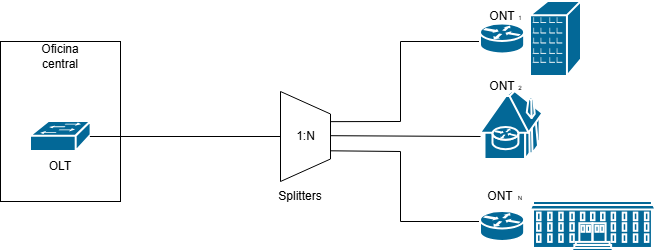
\includegraphics[width=0.8\textwidth]{Esquemas e imágenes/Esquema FTTH.png}
        \caption{Infraestructura de red FTTH}
        \label{fig:FTTH}
    \end{figure}

    \begin{itemize}
        \item OLT (Optical Line Terminal): Es el equipo activo principal ubicado en la central telefónica del proveedor de servicio. Actúa como el concentrador principal que inyecta la señal
         óptica hacia la red de distribución. La OLT es una fuente crítica en la medición de datos, ya que registra el estado de los puertos PON, las caídas masivas y las alarmas de sistemas que son capturados por el
        sistema de monitoreo de red (NOC).
        \item ODN (Optical Distribution Network): Corresponde a la red de planta externa compuesta por el cableado de fibra óptica y divisores ópticos pasivos (splitters). Es en este segmento físico continuo
        donde ocurre la mayor parte de las anomalías que el proyecto busca predecir, tales como atenuaciones por curvaturas, microcortes, empalmes defectuosos o degradaciones del material.
        \item ONT (Optical Network Terminal): Es el dispositivo activo situado en el domicilio del cliente, encargado de convertir la señal óptica en pulsos eléctricos utilizables (Ethernet, Wi-Fi). En el contexto analítico de este proyecto, las ONT actúan como
        los sensores de la última milla, proveyendo registros históricos de las potencias ópticas de recepción ($R_x$) y transmisión ($T_x$), fundamentales para evaluar una posible falla.   
    \end{itemize}


    \subsection{Acercamiento a la solución}
    \noindent
    Para dar respuesta a las limitaciones del actual modelo de mantenimiento reactivo, proponemos el diseño y desarrollo de una arquitectura analítica basada en Aprendizaje Automático. El sistema actuará como una capa
    de inteligencia operativa que complementa a la infraestructura a la red existente, procesando los registros históricos sin necesidad de intervenir físicamente la planta externa.\\\\

    \noindent
    A nivel tecnológico, la solución contempla la construcción de un pipeline de datos estructurado en fases secuenciales. Inicialmente, se implementará un proceso de extracción y limpieza de las diversas fuentes de datos crudos
    provenientes de las ONT, las OLT, los registros del sistema de monitoreo de red (NOC), entre otros. Posteriormente, mediante técnicas de Minería de datos, se extraerán patrones de comportamiento y
    fluctuaciones en la potencia óptica ($R_x$ y $T_x$) para alimentar diversos algoritmos. Esto permitirá generar un índice probabilístico de falla por segmento de red, entregando información procesable que garantice escalabilidad y flexibilidad
    en la toma de decisiones corporativas.\\\\
    
    

    \noindent
    \textbf{Elementos relevantes:}
    \begin{itemize}
        \item \textbf{Usuario:} El usuario principal directo corresponde a ingenieros de operaciones y equipo de mantenimiento de Liberty Latinamerica, quienes recibirán por notificación o correo reportes
        predictivos para gestionar personal encargado del mantenimiento preventivo. Como usuarios secundarios o beneficiarios indirectos se encuentran los clientes finales, quienes experimentarán una mejora sustancial en la QoE
        y QoS al reducir los tiempos de indisponibilidad y las incidencias técnicas.
        \item \textbf{Producto:} El producto consiste en un pipeline y un modelo predictivo de Machine Learning capaz de procesar los datos históricos estructurados para anticipar anomalías y degradaciones en la red de acceso FTTH. Su salida
        principal es una alerta preventiva adjunto a su probabilidad de falla asociada a equipos y segmentos específicos de la red, lo que permitirá a la gerencia tomar decisiones informadas sobre el despliegue de recursos técnicos para el mantenimiento preventivo.
        \item \textbf{Valor agregado:} El contexto de aplicación se enmarca en la industria de las telecomunicaciones y la gestión de infraestructura de proveedores de servicio de internet (ISP). Se orienta hacia el nicho de mantenimiento predictivo
        inteligente, en colaboración directa con actores corporativos de Liberty Latinamerica para validar la solución en un entorno operativo real, priorizando la eficiencia técnica sobre la comercialización del producto. 
    \end{itemize}


    \newpage
\subsection{Estado del Arte}
\noindent
El escenario actual de la gestión de infraestructuras de telecomunicaciones exhibe una transición crítica desde la reparación reactiva hacia la automatización y la inteligencia operativa. La revisión de la literatura académica reciente y de los marcos de trabajo implementados por referentes de la industria evidencia que el uso de algoritmos 
de \textbf{Machine Learning} (ML) se ha consolidado como la principal estrategia técnica para asegurar la confiabilidad en las Redes Ópticas Pasivas (PON).

\subsubsection{Confiabilidad de Red y Gestión Automatizada}
Revisiones sistemáticas sobre la confiabilidad en la industria de las telecomunicaciones coinciden en que la gestión tradicional de la infraestructura de fibra óptica es ineficiente frente a las exigencias modernas de disponibilidad 
\textbf{five-nines uptime} \cite{slr_reliability}. La investigación actual respalda la implementación de modelos de autodiagnóstico avanzados, tales como \textbf{Infinite Multivariate Categorical Mixture Models} \cite{infinite_mixture}, así como marcos automatizados de gestión de infraestructura física en redes FTTH GPON \cite{automated_gpon}, los cuales permiten a la red identificar anomalías físicas y lógicas de forma casi autónoma. Estos estudios establecen el fundamento teórico de que la telemetría pasiva contiene patrones suficientes para inferir el estado de salud de la red sin necesidad de costosas intervenciones físicas exploratorias.

\subsubsection{Tratamiento de Datos Desbalanceados mediante Modelos de Ensamble}
Uno de los mayores desafíos técnicos documentados en el entrenamiento de algoritmos para predicción de anomalías es la naturaleza asimétrica de los datos operativos (\textbf{Imbalanced Data}). En una red FTTH real, los registros históricos de funcionamiento óptimo superan abrumadoramente a los incidentes de falla. 
Para mitigar este sesgo analítico, el estado del arte propone la utilización de Modelos de Ensamble Apilados (\textbf{Stacking Ensemble ML-Based Models}) \cite{stacking_ensemble}. Estas técnicas combinan múltiples algoritmos de clasificación predictiva para aumentar la sensibilidad algorítmica frente a eventos minoritarios (las caídas de servicio), garantizando que el modelo sea capaz de aprender de los síntomas tempranos de degradación sin que la estadística general minimice la alerta.

\subsubsection{Explicabilidad Algorítmica (XAI) en Entornos Operativos}
En el ámbito corporativo, predecir una falla carece de utilidad práctica si el modelo opera como una ``caja negra''. Para abordar esto, la literatura reciente aplica técnicas de interpretabilidad o XAI (\textbf{Explainable AI}), como SHAP (\textbf{Shapley Additive exPlanations}) y 
LIME (\textbf{Local Interpretable Model-agnostic Explanations}) \cite{shap_lime}. Estas metodologías se están incorporando en el análisis de redes FTTH para cuantificar el peso matemático exacto que cada variable (por ejemplo, variaciones de potencia Rx o tasas de cortes) tiene sobre la probabilidad final de degradación, permitiendo que en el área de operaciones comprenda y confíe en la predicción.

\subsubsection{Perspectiva Industrial: Transición Analítica de la Detección a la Prevención}
Desde la perspectiva aplicada de proveedores tecnológicos y plataformas operativas, tales como Nokia \cite{nokia_predictive} y VC4 \cite{vc4_predictive}, el éxito del mantenimiento preventivo no radica exclusivamente en el algoritmo, sino en un proceso robusto de \textbf{Feature Engineering} fundamentado en el conocimiento topológico.
Las herramientas actuales correlacionan registros de estado, alarmas lógicas y desviaciones en los presupuestos de potencia (\textbf{link loss budgets}) a lo largo del tiempo. La identificación temprana de atenuaciones progresivas permite a los operadores despachar personal técnico para prevenir cortes de filamentos debido a tensiones mecánicas o microcurvaturas antes de que afecten los Acuerdos de Nivel de Servicio (SLA) de la compañía.

\subsubsection{Evaluación de Arquitecturas GPON y Aplicación Práctica en ISPs}
Además de los enfoques puramente algorítmicos, la correcta evaluación e implementación de la capa física en redes de acceso FTTH basadas en GPON es un prerrequisito fundamental. Estudios recientes detallan cómo el diseño óptimo de la red y el análisis de la atenuación pasiva condicionan el éxito de cualquier capa analítica superpuesta \cite{ftth_gpon_design}. En esta misma línea, investigaciones aplicadas directamente en los ISP confirman que el uso de \textbf{Machine Learning} en redes de fibra óptica permite detectar variaciones sutiles antes de la disrupción del 
servicio, validando la viabilidad del mantenimiento predictivo en entornos operativos \cite{isp_predictive}.

\subsubsection{Síntesis para la Arquitectura Propuesta}
Si bien la literatura actual establece bases teóricas sólidas, gran parte de las investigaciones académicas se desarrollan sobre datasets simulados o 
entornos altamente controlados. La principal diferencia y el valor agregado de esta propuesta radica en su enfoque directamente operativo e industrial.
A diferencia de los enfoques genéricos existentes, este proyecto no solo implementa técnicas para compensar el desbalanceo de clases y extraer características temporales,
sino que lo hace enfrentándose a la telemetría real y ruidosa de los sistemas de Liberty Latinamerica.\\\\

\noindent
Además, la arquitectura propuesta trasciende la mera predicción algorítmica al cerrar el ciclo de mantenimiento:
integra las probabilidades de falla calculadas con plataformas de ticketing
corporativas, traduciendo la explicabilidad algorítmica (XAI) en alertas preventivas accionables,
resolviendo así la problemática del mantenimiento reactivo en un operador a gran escala con una solución técnica lista para su evaluación en terreno. 

 

    \section{Requisitos del Sistema:}  

        \subsection{\textbf{Requerimientos Funcionales:}}
                    \begin{itemize}
                        \item \textbf{RF1.} Extracción de datos: El sistema debe ser capaz de cargar y leer múltiples archivos de datos estructurados.
                        \item \textbf{RF2.} Limpieza y preprocesamiento: El sistema debe ejecutar ciclos períodicos para limpiar los archivos, específicamente, manejar valores nulos, eliminar datos duplicados, corregir formatos de datos (Por ejemplo, transformar fechas a "dd-MM-yyyy"), filtrar ruido en las mediciones y datos inconsistentes.
                        \item \textbf{RF3.} Feature Engineering: El sistema debe generar nuevas variables calculadas a partir de datos ya procesados (por ejemplo, calcular potencia óptica en diferentes periodos según la medición diaria).
                        \item \textbf{RF4.} Visualización de distribución: Visualizar la distribución de datos mediante gráficos y obtener valores estadísticos para la toma de decisión en la elección de los algoritmos a utilizar.
                        \item \textbf{RF5.} Entrenamiento y validación: El sistema debe permitir entrenar algoritmos de aprendizaje automático utilizando el conjunto de datos históricos previamente procesados y validados según su rendimiento mediante técnicas como \textbf{Cross-validation}.
                        \item \textbf{RF6.} Generación de predicciones: El sistema debe evaluar los nuevos datos ingresados y emitir una probabilidad de degradación o falla por algún equipo (ONT/OLT) en algún segmento de red específico.
                        \item \textbf{RF7.} Evaluación de métricas: El sistema deberá calcular y mostrar métricas de rendimiento del modelo (Por ejemplo, Precisión, Recall, F1-Score, Matriz de confusión, entre otros). 
                        \item \textbf{RF8.} Generación de tickets: El sistema debe comunicarse mediante una API REST con la plataforma Zammad para crear incidencias de mantenimiento de forma automática.
                        \item \textbf{RF9.} Notificación al usuario: El sistema debe enviar alertas estructuradas por correo electrónico al personal técnico detallando el segmento de red en riesgo.
                    \end{itemize}
        \subsection{\textbf{Requerimientos de Interfaces:}}
                    \begin{itemize}
                        \item Interfaz de datos: El sistema requiere de una lectura de archivos locales o en un servicio de nube que soporte los formatos \textbf{.csv}, \textbf{.xlsx} y \textbf{.xls}.
                        \item Interfaz de Salida: El sistema deberá exportar las predicciones generadas a un formato estandarizado (por ejemplo, un archivo \textbf{.csv} con el identificador del equipo y su probabilidad de falla) para que pueda ser interpretado por la gerencia.
                        \item Interfaz de Usuario: Visualizar los resultados mediante un reporte notificado por correo electrónico.
                    \end{itemize}
        \subsection{\textbf{Requerimientos de Ambiente:}}
                    \begin{itemize}
                        \item \textbf{Requerimientos de Software:} 
                        \begin{enumerate}
                            \item Python versión 3.8 o superior.
                            \item Librerías de procesamiento y modelado de datos: Pandas, numpy, matplotlib, Gym, Sckit-learn, XGBoost, pytorch, Tensorflow, dependiendo de las necesidades y arquitectura a escoger.
                            \item Sistema operativo compatible con el entorno de desarrollo (Windows/Linux).
                        \end{enumerate}
                        \item \textbf{Requerimientos de Hardware:}
                        \begin{enumerate}
                            \item \textbf{Memoria RAM:} Se recomienda tener un mínimo de 16 GB o 32 GB de RAM para el procesamiento de datos y unificación de datasets, evitando así, un cuello de botella en la limpieza de varios excels.
                            \item \textbf{Procesamiento (CPU/GPU):} La elección dependerá de la arquitectura de entrenamiento a utilizar. Procesador Multi-núcleo para paralelizar el entrenamiento o tareas de secuencias complejas de pocos núcleos, especialmente útil en técnicas de aprendizaje reforzado de algoritmos como Actor-Crítico (A2C). El uso de la GPU será de gran ventaja en el procesamiento de múltiples hilos ejecutando aritmética básica, siendo especialmente útil en el entrenamiento de redes neuronales profundas. 
                        \end{enumerate}
                        \item \textbf{Entorno de ejecución:} Será necesario requerir un entorno de ejecución en la nube dado un volumen de datos pesado. Por lo que se recomienda contar con una licencia de Google colab (existen otras opciones) que permita seleccionar un hardware con mayor capacidad de cómputo. 
                    \end{itemize}
                


    \section{Planificación del Proyecto}
    \subsection{Objetivo General}
    \noindent
    Desarrollar y validar el pipeline y modelo predictivo basado en algoritmos de aprendizaje automático capaz de anticipar degradaciones físicas en la infraestructura FTTH de Liberty Latinamerica, proporcionando estimaciones probabilísticas
    de falla para optimizar el mantenimiento preventivo y reducir los tiempos de indisponibilidad del servicio, mejorando la experiencia del usuario final y la eficiencia operativa de la compañía.

    \subsection{Objetivos específicos}
    \begin{enumerate}
        \item \textbf{OE1:} Analizar el estado del arte y seleccionar los algoritmos del Aprendizaje automático con mejor desempeño para el procesamiento de datos de redes ópticas y predicción de fallas.
        \item \textbf{OE2:} Desarrollar el pipeline de datos y entrenar los modelos predictivos utilizando los registros históricos de todos los dispositivos y sistema de monitoreo de red.
        \item \textbf{OE3:} Medir y evaluar las métricas de precisión de los modelos entrenados utilizando datasets validados contra el comportamiento histórico de la red real, asegurando su viabilidad para aplicarse en operaciones en terreno.
        \item \textbf{OE4:} Implementar un sistema de notificaciones destinado a los usuarios objetivo que muestre un reporte de incidencia de posibles fallas y estado general de la red.
    \end{enumerate}

    \subsection{Actividades y Milestones}
    \noindent
    

    \subsubsection{Módulo 1: Identificación de técnicas que permitan realizar predicciones}


        \begin{table}[H]
            \centering
            \renewcommand{\arraystretch}{1.5}
            \begin{tabular}{|p{5cm}|p{3cm}|p{2cm}|p{2cm}|p{2cm}|}
            \hline
            \textbf{Actividad} & \textbf{Responsable} & \textbf{Fecha de comienzo} & \textbf{Fecha de término} & \textbf{\% de avance} \\ \hline
            \textbf{OE1: Identificación de técnicas que permitan realizar predicciones} & Gabriel Zapata, Yu Zhou & 22-04-2026 & 20-05-2026 & 100\% \\ \hline
            A1.1: Revisión del estado del arte & Gabriel Zapata, Yu Zhou & 22-04-2026 & 17-05-2026 & 100\% \\ \hline
            T1.1.1: Elaboración de una estrategia de búsqueda & Gabriel Zapata & 22-04-2026 & 11-05-2026 & 100\% \\ \hline
            T1.1.2: Búsqueda de literatura sobre mantenimiento predictivo en redes FTTH & Gabriel Zapata, Yu Zhou & 22-04-2026 & 17-05-2026 & 100\% \\ \hline
            A1.2: Entender la naturaleza de los datos actuales de la FTTH & Gabriel Zapata, Yu Zhou & 22-04-2026 & 20-05-2026 & 100\% \\ \hline
            T1.2.1: ONT & Gabriel Zapata & 22-04-2026 & 20-05-2026 & 100\% \\ \hline
            T1.2.2: PON & Yu Zhou & 22-04-2026 & 20-05-2026 & 100\% \\ \hline
            \end{tabular}
            \caption{Planificación OE1}
            \label{tab:planificacion_avance}
        \end{table}

    \subsubsection{Módulo 2: Entrenar modelos predictivos}



    \begin{table}[H]
            \centering
            \renewcommand{\arraystretch}{1.5}
            \begin{tabular}{|p{5cm}|p{3cm}|p{2cm}|p{2cm}|p{2cm}|}
            \hline
            \textbf{Actividad} & \textbf{Responsable} & \textbf{Fecha de comienzo} & \textbf{Fecha de término} & \textbf{\% de avance} \\ \hline
            \textbf{OE2: Entrenar modelos predictivos} & Gabriel Zapata, Yu Zhou & 20-05-2026 & 20-07-2026 & 31\% \\ \hline
            A2.1: Preparación del pipeline de datos & Gabriel Zapata, Yu Zhou & 20-05-2026 & 15-06-2026 & 47\% \\ \hline
            T2.1.1: Limpieza, normalización y manejo de valores nulos & Gabriel Zapata, Yu Zhou & 20-05-2026 & 25-05-2026 & 70\% \\ \hline
            T2.1.2: Reducción de dimensionalidad & Gabriel Zapata & 25-05-2026 & 29-05-2026 & 35\% \\ \hline
            T2.1.3: Feature engineering & Gabriel Zapata & 29-05-2026 & 04-06-2026 & 35\% \\ \hline
            A2.2: Entrenamiento de modelos candidatos & Yu Zhou & 04-06-2026 & 20-07-2026 & 0\% \\ \hline
            T2.2.1: Optimización de hiperparámetros & Yu Zhou & 04-06-2026 & 20-07-2026 & 0\% \\ \hline
            \end{tabular}
            \caption{Planificación OE2}
            \label{tab:planificacion_avance_oe2}
    \end{table}




    \subsubsection{Módulo 3: Medir los resultados de los modelos en un ambiente real}


    \begin{table}[H]
            \centering
            \renewcommand{\arraystretch}{1.5}
            \begin{tabular}{|p{5cm}|p{3cm}|p{2cm}|p{2cm}|p{2cm}|}
            \hline
            \textbf{Actividad} & \textbf{Responsable} & \textbf{Fecha de comienzo} & \textbf{Fecha de término} & \textbf{\% de avance} \\ \hline
            \textbf{OE3: Medir los resultados de los modelos en un ambiente real} & Gabriel Zapata, Yu Zhou & 10-07-2026 & 20-08-2026 & 0\% \\ \hline
            A3.1: Evaluación estadística & Gabriel Zapata & 10-07-2026 & 24-07-2026 & 0\% \\ \hline
            T3.1.1: Elaboración de matriz de confusión a partir de resultados actuales & Gabriel Zapata & 10-07-2026 & 17-07-2026 & 0\% \\ \hline
            T3.1.2: Cálculo de Precision, Recall y F1 & Gabriel Zapata & 17-07-2026 & 24-07-2026 & 0\% \\ \hline
            A3.2: Evaluación económica & Yu Zhou & 24-07-2026 & 20-08-2026 & 0\% \\ \hline
            T3.2.1: Cálculo de CapEx y OpEx & Yu Zhou & 24-07-2026 & 17-08-2026 & 0\% \\ \hline
            T3.2.2: Estudio de factibilidad del modelo & Yu Zhou & 17-08-2026 & 20-08-2026 & 0\% \\ \hline
            \end{tabular}
            \caption{Planificación OE3}
            \label{tab:planificacion_avance_oe3}
    \end{table}



    \subsubsection{Módulo 4: Desarrollo de sistema de notificaciones}
    \begin{table}[H]
            \centering
            \renewcommand{\arraystretch}{1.5}
            \begin{tabular}{|p{5cm}|p{3cm}|p{2cm}|p{2cm}|p{2cm}|}
            \hline
            \textbf{Actividad} & \textbf{Responsable} & \textbf{Fecha de comienzo} & \textbf{Fecha de término} & \textbf{\% de avance} \\ \hline
            \textbf{OE4: Desarrollo de sistema de notificaciones} & Gabriel Zapata, Yu Zhou & 20-08-2026 & 04-09-2026 & 0\% \\ \hline
            A4.1: Definición del flujo del sistema & Yu Zhou & 20-08-2026 & 22-08-2026 & 0\% \\ \hline
            T4.1.1: Elección de formato de entradas y salidas & Yu Zhou & 20-08-2026 & 21-08-2026 & 0\% \\ \hline
            T4.1.2: Elección de plataforma para la notificación & Yu Zhou & 21-08-2026 & 22-08-2026 & 0\% \\ \hline
            A4.2: Automatización del proceso & Gabriel Zapata, Yu Zhou & 22-08-2026 & 04-09-2026 & 0\% \\ \hline
            T4.2.1: Selección de las herramientas de automatización & Gabriel Zapata, Yu Zhou & 22-08-2026 & 27-08-2026 & 0\% \\ \hline
            T4.2.2: Implementación y prueba del sistema & Gabriel Zapata, Yu Zhou & 27-08-2026 & 04-09-2026 & 0\% \\ \hline
            \end{tabular}
            \caption{Planificación OE4}
            \label{tab:planificacion_avance_oe4}
    \end{table}


    \begin{figure}[H]
            \centering
            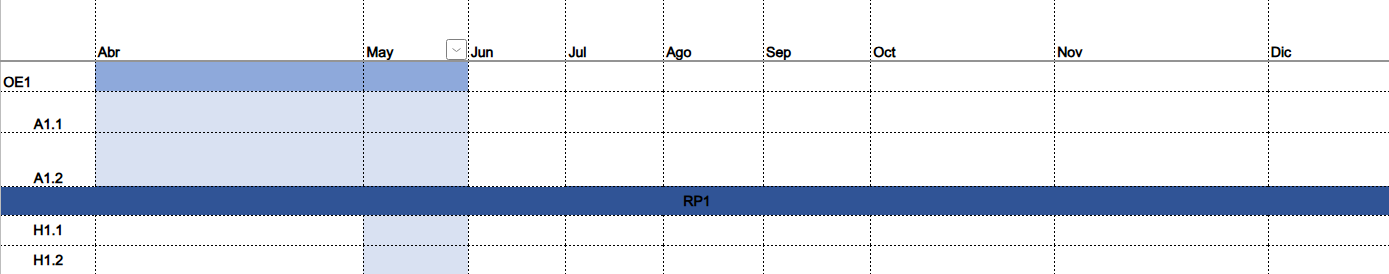
\includegraphics[width=1\textwidth]{Esquemas e imágenes/GANTT1.png}
            \caption{Gantt OE1}
    \end{figure}
    \begin{figure}[H]
            \centering
            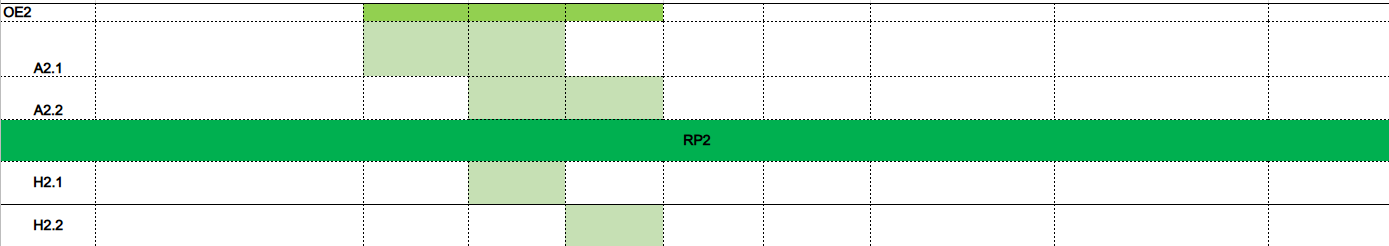
\includegraphics[width=1\textwidth]{Esquemas e imágenes/GANTT2.png}
            \caption{Gantt OE2}
    \end{figure}
    \begin{figure}[H]
            \centering
            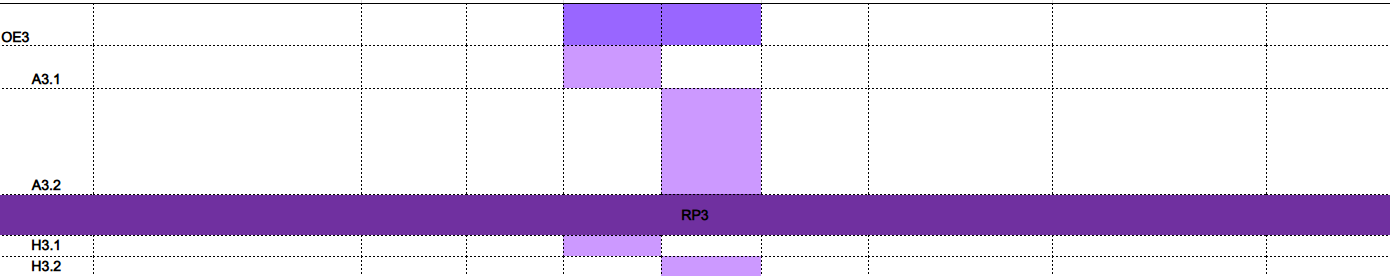
\includegraphics[width=1\textwidth]{Esquemas e imágenes/GANTT3.png}
            \caption{Gantt OE3}
    \end{figure}
    \begin{figure}[H]
            \centering
            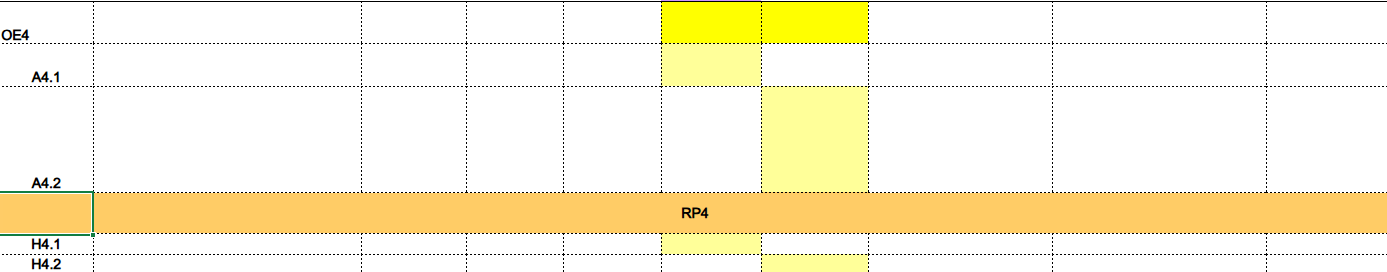
\includegraphics[width=1\textwidth]{Esquemas e imágenes/GANTT4.png}
            \caption{Gantt OE4}
    \end{figure}





\newpage
  \section{Arquitectura del Sistema:}


    \subsection*{\textbf{Diagrama de Contexto}}
    \noindent
    El siguiente diagrama muestra la interacción de los distintos dispositivos con el sistema. Se observa la entrada que recibe el modelo predictivo (Desde las ONT, OLT y NOC) y la 
    salida, en donde realiza una llamada a la API de Zammad para emitir el reporte al equipo de LLA.

    \begin{figure}[H]
            \centering
            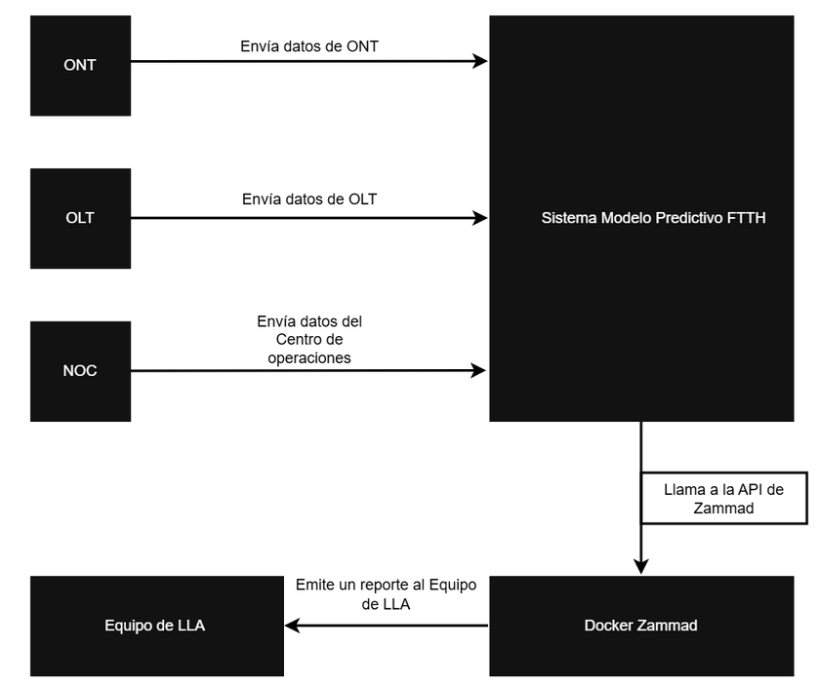
\includegraphics[width=0.6\textwidth]{Esquemas e imágenes/Diagrama Contexto.png}
            \caption{Diagrama de contexto}

    \end{figure}


    \subsection{\textbf{Diagrama de Arquitectura:}} 
    \noindent
    La figura \ref{MODELO ML} resume la arquitectura de alto nivel del modelo predictivo destinado para la posible detección de degradaciones en la red FTTH. La descripción de cada bloque se especifica en el cuadro 5.

                    \begin{figure}[H]
                        \centering
                        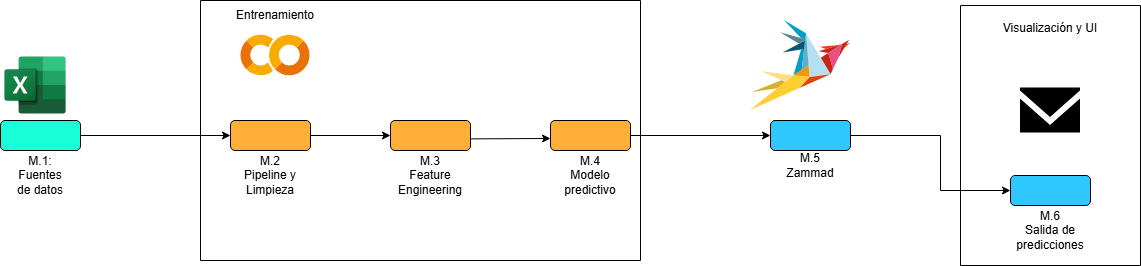
\includegraphics[width=0.8\textwidth]{Esquemas e imágenes/Fases de arquitectura ML.png}
                        \caption{Arquitectura del sistema}
                        \label{MODELO ML}
                    \end{figure}
    \subsection{\textbf{Descripción General de Módulos:}}
                
                    \begin{table}[H]
                        \centering
                        \begin{tabularx}{\textwidth}{|p{3.5cm}|X|p{2cm}|}
                            \hline
                            \rowcolor{black} 
                            \textcolor{white}{Módulos} & \textcolor{white}{Propósito} & \textcolor{white}{Sección}  \\ \hline
                            
                            \textbf{M.1: Fuentes de datos} & El módulo extrae la información de manera estática. Esto incluye: mediciones de potencia óptica (Rx/Tx) provenientes de las ONT, registros de estado de los puertos PON, alarmas, entre otros. & 5.1 \\ \hline
                            \textbf{M.2: Pipeline y Limpieza} & El módulo realiza la consolidación de las distintas fuentes mediante identificadores en común (número serial del dispositivo/ID del cliente y el puerto lógico de la OLT). Además, se realiza una limpieza de datos cuyas acciones incluyen: manejo de valores nulos, registros duplicados y estandarización de formatos. & 5.2 \\ \hline
                            \textbf{M.3: Feature Engineering} & Crea nuevas variables matemáticas a partir de los datos históricos para ayudar al modelo a encontrar patrones de degradación. & 5.3 \\ \hline
                            \textbf{M.4: Modelo predictivo} & Los algoritmos de machine learning (Por ejemplo, Random Forest, XGBoost, Redes neuronales profundas, aprendizaje reforzado). Durante la fase de desarrollo, este componente aprende los patrones de falla. En producción, toma los datos nuevos y calcula la probabilidad de degradación. & 5.4 \\ \hline
                            \textbf{M.5: Integración de Ticketing Zammad} & Actúa como puente automatizado. Recibe las predicciones críticas del modelo e invoca la API de Zammad para registrar formalmente una alerta operativa de mantenimiento. & 5.5 \\ \hline
                            \textbf{M.6: Visualización y UI (Correo electrónico)} & Interfaz final que traduce el ticket generado en un reporte ejecutivo y lo notifica pasivamente al personal técnico mediante correo electrónico. & 5.6 \\ \hline
                        \end{tabularx}
                        \caption{Descripción de cada componente}
                        \label{Tabla MODULO}
                    \end{table}


                
    \subsection{\textbf{Matriz de Requisitos Funcionales y Componentes:}}
                
                    \begin{table}[H]
                        \centering
                        \begin{tabularx}{\textwidth}{|X|p{1cm}|p{1cm}|p{1cm}|p{1cm}|p{1cm}|p{1cm}|}
                            \hline
                            \rowcolor{black} 
                            \textcolor{white}{Requerimiento} & \textcolor{white}{M.1} & \textcolor{white}{M.2} & \textcolor{white}{M.3} & \textcolor{white}{M.4} & \textcolor{white}{M.5} & \textcolor{white}{M.6}  \\ \hline
                            
                            \textbf{RF1} & X & & & & & \\ \hline
                            \textbf{RF2} & & X & & & & \\ \hline
                            \textbf{RF3} & & & X & & & \\ \hline
                            \textbf{RF4} & & & X & X & &  \\ \hline
                            \textbf{RF5} & & & & X & & \\ \hline
                            \textbf{RF6} & & & & X & & \\ \hline
                            \textbf{RF7} & & & & X &  & \\ \hline
                            \textbf{RF8} & & & &  & X & \\ \hline
                            \textbf{RF9} & & & &  &  & X \\ \hline
                        \end{tabularx}
                    \end{table}
    
    \section{Diseño de Módulos del Sistema:}
    \label{sec:modulos}
    \subsection{Fuentes de datos:}

    \begin{itemize}
        \item \textbf{Propósito:} El módulo es el responsable de extraer y recopilar la información cruda de la infraestructura. Este módulo se encarga de reunir por telemetría los datos asociados
        a todos los dispositivos de la red de forma estática y dinámica, incluyendo mediciones de Potencia ($R_x/T_x$), registros de alarma y estado de los puertos PON, entre otros. 

        \item \textbf{Alcance:} Este es el módulo inicial del sistema, encargado de obtener el insumo principal de datos para alimentar el pipeline de procesamiento. 
        
        \item \textbf{Dependencias:}
        
        \begin{itemize}
            \item \textbf{Equipos de red:} Este módulo requiere acceso a los registros exportados provenientes de los dispositivos de red.
        \end{itemize}

        \item \textbf{Supuestos:} Se asume que los sistemas de registro de la empresa no presentarán interrupciones significativas y que la data histórica abarca un periodo suficiente para encontrar patrones.
        \item \textbf{Restricciones:} El módulo debe ser capaz de manejar grandes volúmenes sin consumir recursos computacionales excesivos.
        \item \textbf{Estructura General:}
        \begin{itemize}
            \item \textbf{Entradas:} Archivos estáticos en formato Excel con registros de la red FTTH.
            \item \textbf{Ejecución:} Leer y cargar en memoria los archivos provenientes de la medición de los dispositivos(ONT y OLT) y NOC.
            \item \textbf{Salidas:} Enviar las estructuras de datos crudos (Dataframes) al módulo de pipeline y limpieza.
        \end{itemize}
    \end{itemize}


    \subsection{Pipeline y limpieza:}

    \begin{itemize}
        \item \textbf{Propósito:} Este módulo es el responsable de consolidar las distintas fuentes de información mediante el cruce de identificadores comunes (número serial del dispositivo/ID del cliente y el puerto lógico de la OLT). Además,
         modifica y limpia los datos manejando valores nulos, eliminando duplicados y estandarizando su formato.
        \item \textbf{Alcance:} Actúa como el intermediario fundamental entre los datos en bruto y el procesamiento matemático avanzado.
        \item \textbf{Dependencias:} Depende directamente de la información cruda obtenida por el módulo anterior.
        \item \textbf{Supuestos:} Se asume que el formato de las columnas exportadas desde los sistemas corporativos se mantendrá constante en el tiempo.
        \item \textbf{Restricciones:}
        \begin{itemize}
            \item Las técnicas de limpieza y filtrado de valores nulos no deben alterar significativamente la distribución real de las métricas ópticas.
        \end{itemize}
        \item \textbf{Estructura General:} 
        \begin{itemize}
            \item \textbf{Entradas:} Datos crudos obtenidos del módulo anterior.
            \item \textbf{Ejecución:} 
            \begin{itemize}
                \item Unificar tablas de llaves primarias (identificadores en común).
                \item Filtrar información corrupta, duplicados o datos inconsistentes.
                \item Estandarizar los tipos de datos y formatos.
            \end{itemize}
            \item \textbf{Salidas:} Enviar un conjunto de datos consolidado y limpio al módulo de Feature Engineering.
        \end{itemize}
    \end{itemize}


    \subsection{Feature Engineering}
    \begin{itemize}
        \item \textbf{Propósito:} El módulo es el encargado de crear nuevas variables matemáticas predictivas a partir de los datos históricos. Su objetivo es transformar las métricas aisladas
        en indicadores de tendencia y variación temporal que faciliten al algoritmo encontrar los patrones de degradación física. Además, implementa técnicas de reducción de dimensionalidad para facilitar y optimizar la carga computacional del entrenamiento del
        modelo en el siguiente módulo.
        \item \textbf{Alcance:} Es el paso final de preparación de datos antes del entrenamiento del modelo predictivo.
        \item \textbf{Dependencias:} Requiere el dataset unificado y estandarizado proveniente del módulo de Pipeline y Limpieza.
        \item \textbf{Supuestos:} Se asume que la degradación física en la planta externa tiene un comportamiento temporal progresivo que puede ser capturado mediante el cálculo de tendencias.
        \item \textbf{Restricciones:} La complejidad en el cálculo de las nuevas características (como medias móviles) podría requerir tiempos de ejecución elevados, dependiendo del tamaño del dataset.
        \item \textbf{Estructura General:}
        \begin{itemize}
            \item \textbf{Entradas:} Dataset histórico consolidado y limpio.
            \item \textbf{Ejecución:}
             \begin{itemize}
                \item \textbf{Creación de variables temporales y de agregación:} Se calcularán métricas con sentido físico, tales como: Medias móviles de Potencia de Recepción $R_x$, en ventanas de 7, 14 y 30 días; diferencia temporal de potencia de transmisión $T_x$ respecto a la mediana histórica
                 del puerto; y el conteo acumulado de fluctuaciones o alarmas PON en las últimas 24 y 48 horas.
                \item \textbf{Reducción de dimensionalidad:} Aplicación de técnicas estadísticas PCA, o análisis de correlación Pearson para eliminar variables colineales que no aportan una varianza
                explicativa al estado de la red.
            \end{itemize}
        \end{itemize}
        \item \textbf{Salidas:} Se obtiene un Dataframe procesado, enriquecido con características temporales y optimizado dimensionalmente, listo para el entrenamiento. 
    \end{itemize}


    \subsection{Modelo predictivo}
    \label{subsec:modelo}
    \begin{itemize}
        \item \textbf{Propósito:} Este módulo es el encargado de aplicar y entrenar el modelo mediante un conjunto de algoritmos de Machine learning (como Random Forest, XGBoost, regresiones, Kernel machines, aprendizaje reforzado, entre otros) para evaluar y seleccionar el mejor de ellos para predecir
        predecir la probabilidad de degradación en los enlaces FTTH.

        \item \textbf{Alcance:} Abarca desde el consumo del dataset procesado y enriquecido hasta la exportación del modelo matemático ajustado para inferencias futuras.
        \item \textbf{Dependencias:}
        \begin{itemize}
            \item Depende de la calidad y representatividad de las características extraídas en el módulo de Feature Engineering.
        \end{itemize}
        \item \textbf{Supuestos:} Se asume que el dataset histórico contiene suficientes registros etiquetados implícitamente como una falla frente a un abrumador volumen de comportamiento normal.
        \item \textbf{Restricciones:} El entrenamiento debe mitigar el overfitting provocado por el fuerte desbalance de clases propio de las redes operativas.
        \item \textbf{Estructura General:}
        \begin{itemize}
            \item \textbf{Entradas:} Dataframe limpio con las variables enriquecidas.
            \item \textbf{Ejecución:}
            \begin{itemize}
                \item Se aplicarán técnicas de remuestreo como SMOTE o ajuste de pesos en la función de pérdida para manejar el desbalance de clases.
                \item Metodología de selección: Se entrenarán modelos candidatos de distintas naturaleza.
                \item Debido al impacto operativo de falsos negativos (fallas no detectadas), el modelo final no se seleccionará por su exactitud, sino aquel que maximice la métrica 
                F1-Score y la sensibilidad del área bajo la curva de precisión ($PR-AUC$) durante la validación cruzada.
            \end{itemize}
            \item \textbf{Salidas:} Archivo serializado que contiene el modelo óptimo entrenado y listo para recibir nuevos datos y emitir predicciones probabilísticas.
        \end{itemize}
    \end{itemize}

    \subsection{Integración con Plataforma de Ticketing (Zammad)}
    \label{subsec:zammad}
    \begin{itemize}
        \item \textbf{Propósito:} Este módulo actúa como el puente de comunicación automatizado entre el Modelo Predictivo y la capa de operaciones. Su función es recibir los hallazgos de degradación del modelo e invocar la API de Zammad para registrar formalmente una alerta de mantenimiento preventivo.
        \item \textbf{Alcance:} Comprende la recepción de los datos del modelo, la estructuración del payload y la comunicación de red con el sistema de Helpdesk.
        \item \textbf{Dependencia:} Depende directamente de las predicciones de probabilidad emitidas por el Módulo 5.4 y de la disponibilidad de la API REST de Zammad.
        \item \textbf{Supuestos:} Se asume que Zammad cuenta con los endpoints configurados para recibir solicitudes automatizadas (peticiones HTTP) sin requerir autenticación manual en cada evento.
        \item \textbf{Restricciones:} El módulo debe contar con una lógica de control para evitar la duplicación de tickets operativos si el modelo detecta repetidamente la misma falla en ventanas de tiempo muy cortas.
        \item \textbf{Estructura General:} 
        \begin{itemize}
            \item \textbf{Entradas:} Identificadores del equipo afectado (Ej. OLT, puerto PON, ONT) y la probabilidad de falla calculada por el modelo predictivo.
            \item \textbf{Ejecución: } 
            \begin{itemize}
                \item Evaluación de la probabilidad frente al umbral crítico predefinido.
                \item Construcción del payload en formato JSON con los datos del equipo y la severidad del riesgo (Probabilidad de falla).
                \item Ejecución de la llamada a la API de Zammad para la apertura del ticket.
            \end{itemize} 
            \item \textbf{Salidas:} Un ticket de incidencia generado exitosamente en la plataforma de gestión de la compañía.
        \end{itemize}
    \end{itemize}

    \subsection{Salida de predicción y Notificación}
    \begin{itemize}
        \item \textbf{Propósito:} Constituye la interfaz directa con el usuario final, encargada de notificar al personal técnico o administrativo de forma pasiva y sin generar fricción cognitiva.

        \item \textbf{Alcance:} Abarca el despliegue del reporte final mediante el envío de un correo electrónico automatizado con los detalles esenciales de la anomalía.
        \item \textbf{Dependencias:} Depende de la correcta generación del ticket en el módulo 5.5 (Zammad), el cual dispara la notificación.
        \item \textbf{Supuestos:} Se asume que el usuario final del área de operaciones tiene acceso regular y conectividad a su bandeja de correo corporativo para recibir y revisar la alerta de manera oportuna.
        \item \textbf{Restricciones:} El formato visual del reporte (correo electrónico) debe ser estrictamente en formato HTML ligero sin requerir la carga de imágenes pesadas o complementos externos, garantizando su correcta y rápida visualización en dispositivos móviles en terreno.
        \item \textbf{Estructura General:} 
        \begin{itemize}
            \item \textbf{Entradas:} Confirmación de creación del ticket en Zammad y metadatos asociados (Ubicación física/lógica).
            \item \textbf{Ejecución:}
            \begin{itemize}
                \item Formateo de la información en una plantilla de correo electrónico estandarizada, priorizando la jerarquía visual de la información crítica.
                \item Inclusión de un resumen que contenga la ubicación exacta del segmento de red degradado, el equipo específico y la probabilidad de falla inminente.
            \end{itemize}
            \item \textbf{Salidas:} Correo electrónico de alerta despachado y entregado en la bandeja de entrada del usuario objetivo.
        \end{itemize}
    \end{itemize}
                

\section{Marco General}
\noindent
Recapitulando, el proyecto consiste en el desarrollo de un modelo predictivo
de Machine Learning para la detección temprana de anomalías en la red FTTH de Liberty Latinamerica, complementando con
un sistema de notificaciones automatizados que traduce las predicciones en alertas accionables
para el personal técnico.  En este hito se consolidó el pipeline desde la extracción de fuentes crudas
hasta un dataset unificado listo para el entrenamiento, se definió y validó la variable objetivo del modelo.

\subsection{Hitos Principales del Proyecto}

\begin{itemize}
    \item \textbf{Hito 1 (definición):} Levantamiento del problema, definición de alcances, requisitos funcionales y de ambiente, revisión del estado del arte
    y arquitectura conceptual de la solución.
    \item \textbf{Hito 2 (diseño detallado):} especificación de los seis módulos del sistema (M.1 Fuentes de datos, M.2 Pipeline y Limpieza, M.3 Feature Engineering, M.4 Modelo Predictivo, M.5 Integración Zammad, M.6 Visualización y UI), diagramas de contexto y arquitectura,
    matriz de requerimientos funcionales y diseño de la interfaz de notificación.
    \item \textbf{Hito 3 (Prototipo):} Implementación funcional de los módulos M.1, M.2 y M.3. Se consolidó 8 de las 13 fuentes de datos en un dataset unificado de 999.766 registros a nivel de ONT por día. Se definió
    la variable objetivo (falla\_optica) con criterio técnico y se validó contra una fuente de monitoreo independiente; se ejecutaron tres iteraciones, evaluados cuantitativamente mediante entrenamientos exploratorios
    que triplicaron la capacidad predictiva medida respecto a la línea base. Adicionalmente, se implementó la integración con la plataforma Zammad (M.5), pendiente de conexión con la salida del modelo. La selección
    del modelo definitivo aún no forma parte del alcance de este hito.
    
    \item Siguiente hito (planificado): Cierre de feature engineeing y reducción de dimensionalidad. Evaluación comparativa
    y selección definitiva del modelo mediante validación cruzada; conexión extremo a extremo entre el modelo predictivo y el sistema de notificaciones. Finalmente queda la evaluación de resultados en condiciones representativas del entorno operativo.
\end{itemize}


\subsection{Revisión de Requerimientos}

\begin{table}[H]
\centering
\small 
\renewcommand{\arraystretch}{1.3}
\begin{tabular}{|p{1.1cm}|p{2.9cm}|p{1.9cm}|p{7.2cm}|}
\hline
\textbf{RF} & \textbf{Descripción} & \textbf{Estado H3} & \textbf{Evidencia / Comentarios} \\
\hline
RF1 & Extracción de datos & Cumplido & Carga de 13 archivos (.csv/.xlsx) desde fuentes ONT, OLT, NOC, infraestructura y soporte. \\
\hline
RF2 & Limpieza y preprocesamiento & Cumplido & Corrección de formatos de fecha, tipificación de identificadores, detección y tratamiento de valores centinela de error, deduplicación por clave primaria. \\
\hline
RF3 & Feature Engineering & Parcialmente cumplido & Tres iteraciones ejecutadas (márgenes ópticos respecto a estándar ITU-T, agregaciones por punto de conexión compartido, indicadores de disponibilidad de fuente). Pendiente: cierre de variables temporales y reducción de dimensionalidad. \\
\hline
RF4 & Visualización de distribución & Cumplido & Análisis exploratorio de distribuciones por variable, cobertura por fuente y tasa de eventos por segmento; utilizado como insumo de las decisiones de diseño del dataset. \\
\hline
RF5 & Entrenamiento y validación & En progreso & Se ejecutaron entrenamientos exploratorios con partición por dispositivo, empleados como instrumento de medición del aporte de cada variable construida. La evaluación comparativa formal mediante validación cruzada y la selección del modelo quedan planificadas para el siguiente hito. \\
\hline
RF6 & Generación de predicciones & En progreso & Los modelos exploratorios emiten probabilidad de falla por registro ONT-día; la formalización del punto de operación (umbral) depende de la selección definitiva del modelo. \\
\hline
RF7 & Evaluación de métricas & En progreso & Se debe obtener matriz de confusión y puntaje F1: pendientes de la selección final del modelo. \\
\hline
RF8 & Generación de tickets & Parcialmente cumplido & Integración con la API REST de Zammad implementada y operativa; pendiente la conexión con la salida del módulo predictivo. \\
\hline
RF9 & Notificación al usuario & Parcialmente cumplido & Flujo de notificación por correo operativo a través de Zammad; pendiente la alimentación del reporte con datos reales del modelo. \\
\hline
\end{tabular}
\caption{Estado de cobertura de los Requisitos Funcionales al Hito 3}
\label{tab:cobertura-rf}
\end{table}
 
\subsubsection*{Requisitos No Funcionales y de Ambiente}
 
\begin{itemize}
    \item \textbf{Formatos de entrada (.csv, .xlsx, .xls):} cumplido. El pipeline procesa ambos formatos sin intervención manual.
 
    \item \textbf{Manejo de volumen:} cumplido. El dataset unificado (999.766 registros $\times$ 99 variables) se procesa íntegramente en memoria en el entorno local, sin requerir infraestructura de Big Data, lo que valida el supuesto S3 declarado en el Hito 2.
 
    \item \textbf{Confidencialidad de la información (R2):} cumplido. El trabajo se realiza sobre identificadores técnicos de equipos y cuentas, sin exposición de datos personales de clientes.
 
    \item \textbf{Preservación de la distribución real en la limpieza:} cumplido. Las técnicas de tratamiento de valores faltantes se aplicaron distinguiendo entre ausencia por error de instrumento y ausencia estructural, documentando ambos casos por separado (véase la sección de Verificación).
\end{itemize}


\subsection{Revisión del Diseño}
 \noindent
La arquitectura de seis módulos definida en el Hito 2 se mantuvo sin modificaciones estructurales. Los ajustes introducidos durante la implementación fueron los siguientes:
\begin{itemize}
 
\item \textbf{Acotamiento de los algoritmos candidatos (M.4):} El Hito 2 planteaba un abanico amplio de algoritmos, incluyendo aprendizaje reforzado y redes neuronales profundas. Tras el análisis de la naturaleza del problema, la lista de candidatos se acotó a familias de modelos apropiadas para clasificación supervisada sobre datos tabulares: regresión logística como línea base, Random Forest y modelos de \textit{gradient boosting} (XGBoost/LightGBM). El aprendizaje reforzado se descartó por corresponder a problemas de decisión secuencial, ajenos a la naturaleza de este caso; las redes profundas se descartaron por su rendimiento comparativamente inferior en datos estructurados frente a los ensambles de árboles. Este acotamiento es consistente con la referencia \cite{stacking_ensemble} del estado del arte, que respalda el uso de modelos de ensamble para datos desbalanceados en redes ópticas. Cabe destacar que se trata de una delimitación del espacio de búsqueda, no de una selección: \textbf{la elección del modelo definitivo no se ha realizado en este hito} y queda supeditada a la evaluación comparativa mediante validación cruzada planificada para la siguiente entrega, conforme al criterio de selección establecido en la sección 5.4 del Hito 2 (maximización de F1-Score y PR-AUC).
 
\item \textbf{Definición operacional de la variable objetivo (M.4):} El Hito 2 no especificaba cómo se etiquetaría un registro como ``falla''. Durante la implementación se determinó que la definición amplia basada en alarmas de severidad crítica resultaba inadecuada para el alcance declarado del proyecto, dado que la mayoría de esos eventos correspondía a cortes de energía en el domicilio del cliente, es decir, causas externas a la red. La definición se refinó a eventos de naturaleza óptica. Esta precisión no altera la arquitectura, pero sí constituye una definición de diseño relevante incorporada en este hito.
 
\item \textbf{Incorporación de un estándar técnico externo como referencia (M.3):} El Hito 2 planteaba la ingeniería de características a partir de tendencias y agregaciones sobre los datos históricos. Durante la implementación se incorporó adicionalmente el estándar ITU-T G.984.2 como referencia externa para la construcción de variables, calculando la distancia de cada medición óptica respecto a los límites físicos especificados para la clase de presupuesto óptico de la red. Esta decisión evita definir umbrales de forma circular a partir de los mismos datos que luego se evalúan, y se alineó con la perspectiva industrial descrita en la sección 1.4.4 del Hito 2, que enfatiza la correlación con presupuestos de potencia (\textit{link loss budgets}).
 
\item \textbf{Alcance del módulo de reducción de dimensionalidad (M.3):} La aplicación de técnicas de reducción se mantiene planificada, pero su ejecución quedó condicionada a la selección definitiva del algoritmo, dado que su pertinencia depende del modelo: los ensambles de árboles toleran variables correlacionadas sin degradación, mientras que los modelos lineales sí requieren tratamiento de colinealidad.
 
\end{itemize}

\subsection{Entorno de Soporte y Desarrollo}
 
\begin{itemize}
    \item \textbf{Lenguaje y entorno de ejecución:} Python 3.x sobre entorno virtual local, con Jupyter Notebook como interfaz de desarrollo y documentación del pipeline.
 
    \item \textbf{Librerías de procesamiento de datos:} \texttt{pandas} (manipulación y unificación de tablas) y \texttt{numpy} (operaciones numéricas y tratamiento de valores faltantes).
 
    \item \textbf{Librerías de modelado y evaluación:} \texttt{scikit-learn} (modelos de línea base, particionamiento por grupos, métricas de evaluación y codificación de variables categóricas), \texttt{imbalanced-learn} (técnicas de remuestreo para clases desbalanceadas, específicamente SMOTENC para conjuntos con variables nominales) y \texttt{LightGBM} (modelo de \textit{gradient boosting}).
 
    \item \textbf{Librerías de visualización y análisis estadístico:} \texttt{matplotlib} para el análisis exploratorio de distribuciones; \texttt{scipy} para pruebas de significancia estadística aplicadas a la evaluación de variables candidatas.
 
    \item \textbf{Fuentes de datos:} 13 archivos estáticos en formato \texttt{.csv} y \texttt{.xlsx}, provenientes de los sistemas de ONT y OLT, el sistema de gestión de alarmas, el sistema geoespacial de infraestructura y el registro de contactos de soporte al cliente. El dataset unificado resultante se persiste localmente para evitar la reejecución completa del pipeline en cada sesión de trabajo.
 
    \item \textbf{Referencia normativa externa:} estándar ITU-T G.984.2 (tablas de niveles de potencia óptica para clases B+ y C+), utilizado en la construcción de variables del módulo M.3.
 
    \item \textbf{Plataforma de notificación:} Zammad desplegado en contenedor Docker, con integración vía API REST ya operativa.
 
    \item \textbf{Hardware de desarrollo:} equipo local con procesador multinúcleo, suficiente para el procesamiento del volumen actual de datos y el entrenamiento de los modelos de ensamble evaluados hasta la fecha. No se requirió recurrir a entornos de cómputo en la nube, confirmando el supuesto S3 del Hito 2.
\end{itemize}


\section{Revisión del Prototipo}
\subsection{Contexto General del prototipo}
\noindent
El prototipo desarrollado en este hito implementa la cadena de procesamiento de datos del sistema, esto es, el trayecto que va desde los archivos crudos exportados por los sistemas de Liberty Latinamerica hasta
un conjunto de datos consolidado, enriquecido y apto para el entrenamiento de modelos predictivos. Dicha cadena comprende la extracción de las fuentes (M.1), su limpieza y unión bajo una observación en común (M.2), y la construcción de
variables derivadas (M.3).\\\\

\noindent
La arquitectura completa definida en el Hito 2 contempla, además, una serie de acciones que traducen la salida del modelo en una alerta operativa: modelo predictivo (M.4) $\rightarrow$ una generación de ticket Zammad (M.5) $\rightarrow$ notificación por correo electrónico (M.6).
El módulo de modelado opera sobre el dataframe final y la integración con Zammad es funcional. Sin embargo, la conexión en ambos lados no ha sido establecida, dado que requiere la selección del modelo.\\\\

\noindent
En consecuencia, el prototipo permite hoy ejecutar de extremo a extremo la transformación de datos crudos en un conjunto listo para el entrenamiento y evaluar cuantitativamente el aporte predictivo de cada variable
construida, pero no la emisión automática de alertas a partir de predicciones reales.


\subsection{Esquema General de Componentes del Prototipo}

\begin{itemize}
    \item \textbf{Cadena de datos operativo (M.1 $\rightarrow$ M.2 $\rightarrow$ M.3):} Procesa las 13 fuentes disponibles, realiza la unión de 8 de ellas en un conjunto de 999.766 registros con 99
    variables a nivel de ONT por día, y construye las variables derivadas evaluadas en este hito. El proceso es reproducible desde el estado inicial.

    \item \textbf{Variable objetivo:} La variable objetivo (falla\_optica) se construye a partir del texto de alarma del archivo núcleo, restringida a eventos de naturaleza óptica, siendo contrastada con una fuente de monitoreo independiente.
    
    \item \textbf{Modelado:} Se ejecuta entrenamientos con Random Forest y LightGBM, como instrumento de medición del aporte a las variables construidas. No se ha seleccionado un modelo definitivo ni establecido un punto de operación.
    
    \item \textbf{Integración de Ticketing (M.5):} La comunicación con la API REST Zammad se encuentra implementada sobre una instancia desplegada en contenedor Docker, a la espera de recibir las predicciones.
    
    \item \textbf{Notificación (M.6):} Se encuentra disponible el flujo de envío de correo a partir del ticket generado. 
\end{itemize}



\subsection{Descripción de Componentes}
\noindent
A continuación se describen los componentes implementados, su interacción, fundamento teórico, elementos tecnológicos y funciones principales, en correspondencia con la definición de los módulos de la sección 5.

\subsubsection*{(a) Fuentes de datos (M.1)}
 
\begin{itemize}
    \item \textit{General}: carga de los archivos exportados desde los sistemas de medición de Liberty Latinamerica respecto a dispositivos ONT y OLT, el sistema de gestión de alarmas, el sistema geoespacial de infraestructura y el registro de contactos de soporte.
    \item \textit{Interacción}: entrega las estructuras de datos crudos al módulo de pipeline y limpieza, sin transformación previa.
    \item \textit{Marco teórico}: la medición pasiva de la red contiene información suficiente para inferir el estado de salud de la infraestructura sin intervención física exploratoria.
    \item \textit{Elementos tecnológicos}: \textbf{pandas} para la lectura de archivos en formato \textbf{.csv} y \textbf{.xlsx}.
    \item \textit{Funciones}: cargar cada fuente preservando su estructura original, registrar el número de registros leídos por archivo y verificar la presencia de las columnas declaradas en el esquema.
\end{itemize}


\subsubsection*{(b) Pipeline y limpieza (M.2)}
 
\begin{itemize}
    \item \textit{General}: consolida las fuentes en un único conjunto de datos con unidad de observación ONT-día, corrige inconsistencias de formato y trata los valores ausentes según su origen.
    \item \textit{Interacción}: recibe las estructuras crudas de M.1 y entrega el conjunto consolidado a M.3.
    \item \textit{Marco teórico}: la consolidación se apoya en la topología de la red, empleando como identificadores de cruce la cuenta del suscriptor y la ubicación física del equipo (sitio, chasis, tarjeta y puerto), conforme al esquema de gestión de infraestructura FTTH/GPON descrito en [3]. El tratamiento de valores atípicos adopta un criterio conservador, dado que en un problema de detección de degradaciones la caída abrupta de potencia constituye, estadísticamente, un valor atípico, y su eliminación suprimiría la señal de interés.
    \item \textit{Elementos tecnológicos}: \textbf{pandas} y \textbf{numpy}.
    \item \textit{Funciones}: unifica fuentes con identificadores en común, estandarizar tipos de dato, identificar y anular/tratar los valores excepcionales.
\end{itemize}


\subsubsection*{(c) Feature Engineering (M.3)}
 
\begin{itemize}
    \item \textit{General}: construye variables derivadas a partir del conjunto unificado, con el propósito de expresar las mediciones en términos que faciliten al algoritmo la identificación de patrones de degradación.
    \item \textit{Interacción}: recibe el conjunto consolidado de M.2 y entrega el conjunto enriquecido a M.4.
    \item \textit{Marco teórico}: la construcción de variables se fundamenta en el conocimiento topológico y en la desviación respecto de los presupuestos de potencia óptica (\textbf{link loss budgets}), conforme a la perspectiva industrial descrita en [6], [7]. Los límites de dichos presupuestos se toman del estándar ITU-T G.984.2, lo que evita definirlos de forma circular a partir de los mismos datos que posteriormente se evalúan. Adicionalmente, se incorporan variables de agregación por punto de conexión compartido, dado que en una arquitectura PON los equipos conectados a un mismo puerto comparten el tramo de distribución óptica.
    \item \textit{Elementos tecnológicos}: \textbf{pandas}, \textbf{numpy} y \textbf{scipy} para las pruebas de significancia aplicadas a la evaluación de variables candidatas.
    \item \textit{Funciones}: calcular el margen de cada medición óptica respecto de los límites del estándar, construir variables adicionales a nivel de puerto de conexión compartido; generar indicadores de disponibilidad por fuente; y evaluar el aporte de cada variable construida mediante contraste estadístico.
\end{itemize}

\subsubsection*{(d) Modelo predictivo (M.4)}
 
\begin{itemize}
    \item \textit{General}: entrena algoritmos de clasificación sobre el dataframe final y estima la probabilidad de falla óptica por registro. En el estado actual opera en modalidad exploratoria.
    \item \textit{Interacción}: utiliza el dataframe por M.3. Su salida está destinada a M.5, conexión aún no establecida.
    \item \textit{Marco teórico}: el desbalance de clases propio de los datos operativos de red exige técnicas específicas, siendo los modelos de ensamble la estrategia respaldada por la literatura para este tipo de problema [4]. La evaluación se basa en métricas definidas sobre la clase minoritaria, dado que la exactitud resulta inadecuada ante una prevalencia del 0,516\,\%.
    \item \textit{Elementos tecnológicos}: \textbf{scikit-learn}, \textbf{imbalanced-learn} (SMOTENC) y \textbf{LightGBM}.
    \item \textit{Funciones}: particiona el conjunto respetando la agrupación por dispositivo, aplicar técnicas de tratamiento del desbalance, entrenar los modelos candidatos (en fase exploratoria) y estimar métricas de desempeño.
\end{itemize}

\subsubsection*{(e) Integración de ticketing (M.5)}
 
\begin{itemize}
    \item \textit{General}: traduce las predicciones que superan el umbral de decisión dentro de la plataforma de gestión de la empresa.
    \item \textit{Interacción}: recibirá los identificadores del equipo afectado y la probabilidad estimada desde M.4, y notificará a M.6 la creación del ticket.
    \item \textit{Marco teórico}: el valor del mantenimiento predictivo depende de que la salida analítica se integre al flujo de trabajo existente.
    \item \textit{Elementos tecnológicos}: Zammad desplegado en contenedor Docker y comunicación mediante API REST.
    \item \textit{Funciones}: evalúa la probabilidad frente al umbral vigente, construye el payload (API Zammad) con los identificadores del equipo y la severidad asociada e invoca la creación del ticket.
\end{itemize}


\subsubsection*{(f) Salida de predicción y notificación (M.6)}
 
\begin{itemize}
    \item \textit{General}: constituye la interfaz con el usuario final, mediante el envío de un reporte por correo electrónico a partir del ticket generado.
    \item \textit{Interacción}: se activa a partir de la creación del ticket en M.5.
    \item \textit{Marco teórico}: la comunicación de la predicción debe incorporar los elementos que permitan al personal técnico evaluar su pertinencia.
    \item \textit{Elementos tecnológicos}: Contiene un sistema de notificación por correo de Zammad, contenido en formato HTML ligero sin recursos externos para su correcta visualización en dispositivos móviles.
    \item \textit{Funciones}: formatea el reporte priorizando la jerarquía visual de la información crítica, e incluye la ubicación del segmento afectado, el equipo específico y la probabilidad estimada de falla.
\end{itemize}

\subsection{Interfaces Implementadas en el Prototipo}
 
El sistema no contempla una interfaz gráfica para la operación del modelo, dado que su salida se consume a través de la plataforma de \textbf{ticketing}. En consecuencia, las interfaces del prototipo corresponden a la salida de notificación destinada al usuario final.\\\\

\noindent
La integración con la plataforma de \textbf{Ticketing} se encuentra operativa sobre una instancia de Zammad desplegada en un contenedor Docker. La figura \ref{fig:Zammad1} muestra el historial de incidencias generadas mediante la API REST,
lo que evidencia el funcionamiento del mecanismo de creación automática de tickets especificado en el RF8.

\begin{figure}[H]
    \centering
    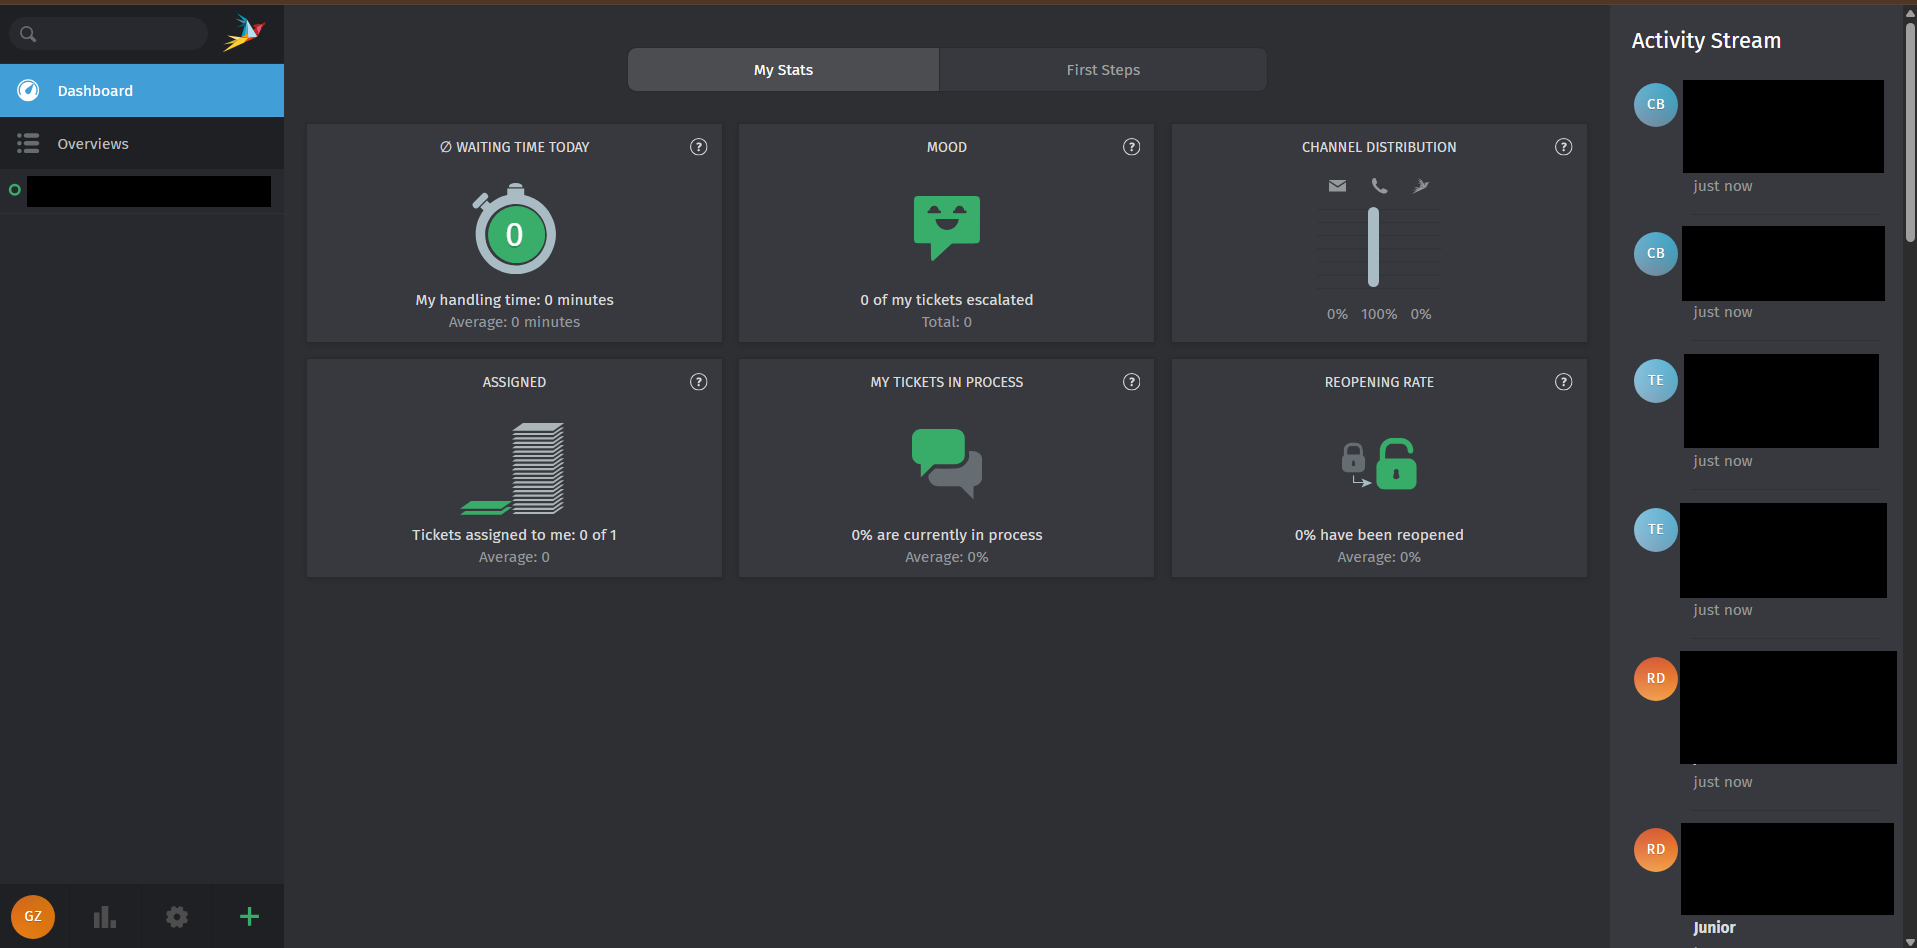
\includegraphics[width=0.8\textwidth]{Esquemas e imágenes/ZAMMAD1.png}
    \caption{Interfaz Historial de tickets Zammad}
    \label{fig:Zammad1}
\end{figure}

El envío de la notificación por correo electrónico fue verificado de manera preliminar durante las pruebas de integración, si bien no se dispone de registro documental de dicha ejecución en el presente informe. Su configuración
definitiva requiere el uso de una cuenta de correo destinada al entorno de pruebas, tarea contemplada para la siguiente entrega junto con los casos de los planes de prueba.



\section{Verificación, Validación y Testing}
\label{sec:vvt}
\noindent
verificación determina si los productos de cada etapa del desarrollo satisfacen los requisitos y 
 especificaciones establecidos para dicha etapa; en el contexto de este proyecto, si cada módulo implementa
  correctamente su diseño. La validación determina si el sistema resultante satisface el uso previsto 
  y las necesidades del usuario; en este caso, si las alertas generadas permiten a Liberty Latinamerica anticipar
   degradaciones físicas en la red FTTH con una precisión que justifique el mantenimiento preventivo de la fibra.\\

\subsection{Verificación}
\label{subsec:verificacion}

\noindent
La verificación tiene por objetivo demostrar que los datos que ingresan al modelo corresponden exactamente
 a lo especificado en el diseño. Los defectos en la limpieza rara vez producen
  errores de ejecución. No obstante, generan conjuntos de datos estructuralmente válidos pero con contenido incorrecto
  , que el modelo va incorporar de manera posterior provocando resultados defectuosos. Por este motivo, la verificación se define en
   las siguientes etapas que se describen a
    continuación.\\
    \newline
\noindent
\textbf{Carga de datos } 
\\
Cada fuente de datos se importa, se filtra a registros de Panamá mediante el prefijo \texttt{PAN} del identificador de sitio, y se perfila mediante 
la fracción de valores nulos por columna. El Cuadro~\ref{tab:carga} resume los volúmenes que reporta el notebook antes
y después de la limpieza. Además, se descartan las líneas mal formadas y se contabilizan el número de estas por archivo.

\begin{table}[htbp]
\centering
\caption{Volumen de registros por fuente según el notebook de minería de datos}
\label{tab:carga}
\small
\renewcommand{\arraystretch}{1.25}
\begin{tabularx}{\textwidth}{|p{6.1cm}|r|>{\raggedleft\arraybackslash}p{2.5cm}|X|}
\hline
\rowcolor{black}
\textcolor{white}{\textbf{Fuente}} & \textcolor{white}{\textbf{Cargados}} & \textcolor{white}{\textbf{Tras limpieza}} & \textcolor{white}{\textbf{Rol}} \\ \hline
\texttt{mosaic\_\allowbreak{}ont\_\allowbreak{}sts\_\allowbreak{}cwp.csv} & 1.000.000 & 999.766 & Núcleo (\texttt{serial} + \texttt{dt}) \\ \hline
\texttt{bbms\_\allowbreak{}portstats.csv} & 999.953 & 446.357 & Integrada \\ \hline
\texttt{bbms\_\allowbreak{}subscribers\allowbreak{}dump.csv} & 999.941 & 950.222 & Integrada \\ \hline
\texttt{cwp\_\allowbreak{}historic\_\allowbreak{}fixed\_\allowbreak{}network\_\allowbreak{}points.csv} & 990.497 & 990.497 & Integrada \\ \hline
\texttt{cwp\_\allowbreak{}Serviceabily\_\allowbreak{}HFC\_\allowbreak{}FTTH\_\allowbreak{}2024\_\allowbreak{}GAA\_\allowbreak{}2025.csv} & --- & 33.958 (nivel FDP) & Integrada (agregada por OLT) \\ \hline
\texttt{mosaic\_\allowbreak{}pon\_\allowbreak{}sts\_\allowbreak{}cwp.csv} & 1.000.000 & 1.000.000 & Integrada \\ \hline
\texttt{nce.csv} & 999.650 & 407.088 (eventos) & Integrada (agregada por día) \\ \hline
\texttt{pca\_\allowbreak{}wsp\_\allowbreak{}feb\_\allowbreak{}abr\_\allowbreak{}2026\_\allowbreak{}detalle.csv} & 114.183 & 114.110 & Integrada \\ \hline
\texttt{PON.xlsx} & --- & 14.298 (100.086 en formato largo) & Reservada para validación \\ \hline
\texttt{ONT.csv} & --- & 214.751 & Excluida  \\ \hline
\texttt{NOC.csv} & --- & 4.668 & Excluida  \\ \hline
\texttt{mosaic\_\allowbreak{}ont\_\allowbreak{}sts\_\allowbreak{}stats\_\allowbreak{}cwp.csv} & 1.999 & 1.975 & Excluida \\ \hline
\texttt{pca\_\allowbreak{}wsp\_\allowbreak{}feb\_\allowbreak{}abr\_\allowbreak{}2026\_\allowbreak{}agregado.csv} & 385 & 385 & Excluida  \\ \hline
\end{tabularx}
\end{table}

\paragraph{Limpieza por archivo .}
Para asegurar la integridad de los datos, se aplicaron los siguientes tratamientos de limpieza y estandarización:
\begin{itemize}
    \item \textbf{Unicidad de llaves:} Se eliminan los duplicados de  (\texttt{port\_id}, \texttt{dt}) en \texttt{bbms\_portstats}, asimismo en \texttt{cwp\_Serviceabily} verifica cero duplicados por (\texttt{oltid}, \texttt{fdh}, \texttt{fdp}, \texttt{name}). 
    \item \textbf{Eliminación de lecturas físicamente imposibles:} en \texttt{bbms\_portstats} se anulan las potencias iguales a 21.474.836 o con magnitud superior a 60 dBm. En el núcleo se anulan los valores de $-50$ dBm en \texttt{olt\_rx} y \texttt{olt\_tx}, y se marcan como \texttt{lectura\_optica\_atipica} las lecturas con \texttt{olt\_rx} positiva u \texttt{olt\_tx} inferior a $-10$ dBm. En \texttt{ONT.csv} se anulan los contadores BIP superiores a 1.000.000 (indicador \texttt{bip\_overflow\_detectado}) y los tiempos de actividad negativos. En \texttt{mosaic\_ont\_sts\_stats} se descartan los registros del 14 de abril de 2026, cuyos conteos de ONT en servicio, advertencia e interrupción son simultáneamente nulos.
    \item \textbf{Ausencia total frente a ausencia parcial:} cuando todas las mediciones de un grupo están vacías se crea un indicador (\texttt{ont\_sin\_medicion}, \texttt{ont\_sin\_telemetria}, \texttt{ont\_sin\_servicio\_asignado}) y no se ingresa. Cuando la ausencia es parcial, se ingresa la mediana (variables continuas) o la moda (variables categóricas).
    \item \textbf{Fechas en formato mixto:} \texttt{NOC.csv} combina los formatos DD/MM/AAAA y MM/DD/AAAA. Se interpreta como día el primer campo cuando es mayor que 12 y se identifican las fechas ambiguas, en las que ambos campos son menores o iguales a 12.
\end{itemize}


\subsection{Validación}
\label{subsec:validacion}
\noindent
La validación evalúa la adecuación del sistema a la necesidad operativa de Liberty Latinamerica,
 formalizada en los requerimientos RF5 (entrenamiento y validación mediante validación cruzada),
  RF6 (generación de predicciones) y RF7 (cálculo de métricas), así como en el criterio de selección de M.4
   (Sección~\ref{subsec:modelo}), que privilegia el F1-Score y el área bajo la curva de precisión-cobertura (PR-AUC) 
   por sobre la exactitud.

\subsubsection{Validación ejecutada de la variable objetivo}
La definición de \textbf{falla\_optica} se contrastó contra el registro de
alarmas de un sistema de gestión de red independiente del que origina la
variable, aislando en éste los eventos de naturaleza óptica (21.133 registros).
El cruce por dispositivo y día identificó 10.902 registros marcados por ambas
fuentes.\\\\

\noindent
El indicador de validez adoptado no es la coincidencia absoluta, sino el
enriquecimiento: la probabilidad de que un registro esté etiquetado como falla
es del 2,578\,\% cuando el sistema independiente reporta una alarma óptica,
frente a 0,493\,\% cuando no la reporta, lo que equivale a un factor de 5,2.
Dado que ambos sistemas no comparten el sistema en donde son capturado los datos, esta concordancia
constituye evidencia de validez de \textbf{falla\_optica}.\\\\

\noindent
El contraste se repitió admitiendo desfases de hasta dos días entre ambas
fuentes, obteniéndose factores de 5,2 ($\pm$0 días), 4,8 ($\pm$1 día) y 5,4
($\pm$2 días). La ausencia de una tendencia creciente indica que la
concordancia no depende de la tolerancia temporal adoptada.\\\\

\noindent
Adicionalmente, se verificó que la variable es reconstruible de forma
determinista a partir de su columna de origen (no hay discrepancia de los
999.766 registros) y que ninguna variable derivada de dicha columna forma parte
del conjunto de predictores, descartando la fuga de información directamente.

\subsection{Métricas de desempeño.}
En un conjunto en el que la gran mayoría de los registros ONT-día corresponde a operación normal,
 un clasificador que asigne sistemáticamente la clase ``sin falla'' alcanza una exactitud próxima al 100\,\%
  sin detectar degradación alguna. La evaluación se basa, por tanto, en métricas definidas sobre la clase de interés.
   La \textbf{precisión} cuantifica la fracción de alertas emitidas que corresponde a fallas reales, y el
    recall la fracción de fallas reales que fueron alertadas. El F1-Score combina ambas:
\begin{equation}
    F_1 = \frac{2 \cdot P \cdot R}{P + R}
    \label{eq:f1}
\end{equation}
donde:
\begin{itemize}
    \item $P = TP/(TP + FP)$ es la precisión;
    \item $R = TP/(TP + FN)$ es el recall;
    \item $TP$ es el número de registros con falla alertados por el modelo (verdaderos positivos);
    \item $FP$ es el número de registros sin falla alertados por el modelo (falsos positivos);
    \item $FN$ es el número de registros con falla no alertados por el modelo (falsos negativos).
\end{itemize}
Dado que el F1-Score depende del umbral de decisión, se complementa con el PR-AUC, estimado mediante la precisión promedio:
\begin{equation}
    AP = \sum_{n} \left( R_n - R_{n-1} \right) P_n
    \label{eq:ap}
\end{equation}
donde $n$ indexa los umbrales de decisión ordenados de mayor a menor, $P_n$ y $R_n$ son la precisión y el recall obtenidos con el umbral $n$, y $R_0 = 0$. 


\subsection{Plan de Testing}
\label{subsec:testing}
\noindent
El plan de pruebas traduce las actividades anteriores en casos ejecutables. Las pruebas unitarias, de integración y de continuidad operativa.
\\
\noindent
\\
\textbf{Pruebas unitarias.}
\newline
El Cuadro~\ref{tab:unitarias} define los casos  para  las funciones de limpieza.

\begin{table}[H]
\centering
\caption{Casos de prueba unitarios sobre las reglas de limpieza del notebook}
\label{tab:unitarias}
\small
\renewcommand{\arraystretch}{1.3}
\begin{tabularx}{\textwidth}{|p{1.15cm}|p{1.2cm}|X|X|}
\hline
\rowcolor{black}
\textcolor{white}{\textbf{ID}} & \textcolor{white}{\textbf{Sección}} & \textcolor{white}{\textbf{Caso}} & \textcolor{white}{\textbf{Resultado esperado}} \\ \hline
UT-01 & 3.1 & \texttt{uptime\_a\_segundos("19d 4h 38m 14s")} & 1.658.294~s \\ \hline
UT-02 & 3.1 & \texttt{uptime\_a\_segundos} con valor nulo y con componentes omitidos (\texttt{"0d 6h 4m 26s"}) & Valor nulo; 21.866~s \\ \hline
UT-03 & 5.1 & Potencia $R_x$ igual a 21.474.836 y potencia de 75~dBm & Ambos valores anulados \\ \hline
UT-04 & 3.5 & \texttt{olt\_rx} igual a $-50$~dBm; \texttt{olt\_rx} igual a $+1{,}2$~dBm & Valor anulado \texttt{lectura\_optica\_atipica} verdadero \\ \hline
UT-05 & 3.5 & Registro con las cinco mediciones vacías; registro con una sola vacía & \texttt{ont\_sin\_medicion} verdadero sin integración; integración solo del campo vacío \\ \hline
UT-06 & 3.5 & Dos registros con igual (\texttt{serial}, \texttt{dt}), uno con alarma & Se conserva un único registro, el que tiene alarma \\ \hline
UT-07 & 3.10 & Contador BIP igual a 2.475.388.463 & \texttt{bip\_overflow\_detectado} verdadero y valor anulado \\ \hline
UT-08 & 3.9 & \texttt{parsear\_fecha\_noc("30/10/2025")} y \texttt{("3/25/2026")} & 30-10-2025 y 25-03-2026 \\ \hline
UT-09 & 3.9 & \texttt{es\_ambiguo("1/3/2026")} & Verdadero; fecha interpretada documentada \\ \hline
UT-10 & 3.8 & Expresión regular sobre \texttt{"Frame=0, Slot=13, Subslot=65535, Port=7, ONUID=35"} y sobre la misma cadena sin \texttt{ONUID} & (0, 13, 7, 35); \texttt{alarma\_nivel\_card} verdadero \\ \hline
UT-11 & 3.6 & Registro horario con conteos de servicio, advertencia e interrupción iguales a cero & Registro excluido \\ \hline
\end{tabularx}
\end{table}
\noindent
\textbf{Pruebas de integración.}
\newline
Las pruebas de integración verifican el pipeline de datos.

\begin{table}[H]
\centering
\caption{Casos de prueba de integración}
\label{tab:integracion}
\small
\renewcommand{\arraystretch}{1.3}
\begin{tabularx}{\textwidth}{|p{1.15cm}|p{1.9cm}|X|X|}
\hline
\rowcolor{black}
\textcolor{white}{\textbf{ID}} & \textcolor{white}{\textbf{Cadena}} & \textcolor{white}{\textbf{Caso}} & \textcolor{white}{\textbf{Resultado esperado}} \\ \hline
IT-01 & M.1$\rightarrow$M.2 & Ejecución completa del programa desde un núcleo reiniciado, dos veces & Sin errores; 999.766 registros \\ \hline
IT-02 & M.2 & Siete uniones sobre el núcleo & Filas sin cambio y tasa de coincidencia reportada en cada unión \\ \hline
IT-03 & M.2 & Seguimiento de un conjunto de ONT de control desde el archivo de origen hasta \texttt{df\_final} & Identificadores y valores trazables en cada etapa \\ \hline
IT-04 & M.2 & Inspección de columnas de \texttt{df\_final} y de archivos exportados & Ausencia de nombres, direcciones y coordenadas de clientes (R2) \\ \hline
IT-05 & M.4$\rightarrow$M.5 & Predicción superior al umbral para un puerto PON en una instancia de prueba de Zammad & Un ticket con OLT, puerto, severidad y probabilidad \\ \hline
IT-06 & M.4$\rightarrow$M.5 & Predicciones idénticas consecutivas sobre el mismo puerto & Un único ticket (Sección~\ref{subsec:zammad}) \\ \hline
IT-07 & M.5$\rightarrow$M.6 & Ticket generado a partir de una predicción & Correo HTML sin recursos externos, con ubicación, equipo y probabilidad \\ \hline
\end{tabularx}
\end{table}

\textbf{Pruebas de continuidad operativa.} 
\newline
Las pruebas de aceptación se ejecutarán una vez definidos la señal de falla y el modelo. El sistema se plantea ejecutarse de forma secuencial, día a día,  y sus alertas se contrastan con los eventos efectivamente registrados, sin intervención
 sobre el entorno productivo inicialmente. Se contemplan tres casos:
\begin{itemize}
    \item \textbf{CD-01, contraste con eventos registrados:} fracción de eventos de falla precedidos por al menos una alerta y número de alertas por evento, calculados sobre el período de prueba del nivel puerto PON-día.
    \item \textbf{CD-02, revisión experta:} El jefe de operaciones (tutor) examina una muestra de alertas estratificada por severidad, que incluye falsos positivos, y registran si cada una es accionable. Esta revisión valida simultáneamente las interpretaciones de campos señaladas en la Sección~\ref{subsec:validacion}.
    \item \textbf{CD-03, legibilidad del reporte:} el usuario recibe la notificación en su dispositivo móvil y se registra si identifica equipo, ubicación y severidad sin información adicional.
\end{itemize}
Los criterios de aceptación de estas pruebas dependen de la capacidad operativa de Liberty Latinamerica, por lo que serán acordados con el tutor antes de su ejecución. 

\subsection{Análisis Crítico y Evaluación de Riesgos}
\label{subsec:riesgos_tecnicos}
\noindent
Los riesgos P1 a P3, descritos en la Sección~\ref{subsec:riesgos}, corresponden a riesgos de gestión del proyecto. El Cuadro~\ref{tab:riesgos_tecnicos} los sintetiza junto con su probabilidad e impacto estimados, las medidas de mitigación y el indicador de seguimiento.

\begin{table}[htbp]
\centering
\caption{Riesgos técnicos de implementación (P: probabilidad, I: impacto, A: alta, M: media, B: baja)}
\label{tab:riesgos_tecnicos}
\small
\renewcommand{\arraystretch}{1.3}
\begin{tabularx}{\textwidth}{|p{0.9cm}|X|p{0.4cm}|p{0.4cm}|X|X|}
\hline
\rowcolor{black}
\textcolor{white}{\textbf{ID}} & \textcolor{white}{\textbf{Riesgo}} & \textcolor{white}{\textbf{P}} & \textcolor{white}{\textbf{I}} & \textcolor{white}{\textbf{Mitigación}} & \textcolor{white}{\textbf{Indicador}} \\ \hline
RT1 & Cobertura temporal insuficiente de la telemetría de ONT & A & A & Solicitar extractos de varios meses (D1). Validar la predicción a nivel de puerto PON & Días de historia por fuente \\ \hline
RT2 & Señal de falla contaminada por eventos no ópticos & A & A & Taxonomía de alarmas validada por el tutor. Contraste con \texttt{PON.xlsx} & Correlación de rangos con la fuente independiente \\ \hline
RT3 & Exposición de datos personales (R2) & B & B & Eliminar \texttt{service\_address}. Agregar el mapa a nivel de OLT & Prueba IT-04 \\ \hline
RT4 & Fuga de información en la evaluación & M & A & Partición temporal agrupada por puerto. Exclusión de variables derivadas de la etiqueta & Diferencia entre desempeño de validación y de prueba \\ \hline
RT5 & Distorsión de la distribución óptica. & M & A & Cuantificar la fracción de datos reemplazados & Fracción de datos reemplazados por columna \\ \hline
RT6 & Uniones sin coincidencia no detectadas & M & M & Tasa de coincidencia por unión & Prueba IT-02 \\ \hline
RT7 & Ejecución no reproducible del programa & M & M & Ejecución completa desde núcleo reiniciado. & Prueba IT-01 \\ \hline
RT8 & Interpretación incorrecta de campos sin diccionario (D2) & M & M & Validación de umbrales y significados con el operador & Decisiones validadas / decisiones totales \\ \hline
RT9 & Falsos positivos y fatiga de alertas & A & A & Agregación por puerto PON. Umbral según capacidad de despacho. Control de duplicados en M.5 & Precisión operativa de los tickets \\ \hline
\end{tabularx}
\end{table}


\section{Gestión de Riesgos:}
    \label{sec:riesgos}

        \subsection{\textbf{Supuestos:}}
                    \begin{itemize}
                        \item \textbf{S1-Correlación de variables:} Se asume que existe una correlación matemática real y detectable entre los parámetros de telemetría extraídos y las degradaciones físicas de la red antes de que se conviertan en un reclamo masivo por parte de los clientes.
                        \item \textbf{S2-Representatividad histórica:} Se asume que los archivos Excel/CSV entregados por la jefatura contienen un historial de tiempo lo suficientemente amplio (muchos meses) para que el algoritmo pueda aprender los patrones estacionales y transitorios de las fallas.
                        \item \textbf{S3-Capacidad de procesamiento:} Se asume que los datos proporcionados podrán ser procesados con los recursos computacionales actuales sin requerir de una infraestructura de Big Data de alto costo.
                    \end{itemize}
        \subsection{\textbf{Dependencias:}}
                    \begin{itemize}
                        \item \textbf{D1-Entrega de datos corporativos:} El avance del cronograma depende estrictamente de que el tutor y Liberty Latinamerica proporcionen los datasets iniciales y las actualizaciones de datos en los plazos acordados.
                        \item \textbf{D2-Diccionario de datos:} Se depende de la empresa para la entrega de un glosario o diccionario de datos que explique el significado de cada columna en los archivos Excel para realizar un Feature Engineering y una reducción de dimensionalidad correctas.
                        \item \textbf{D3-Validación experta:} Se depende del conocimiento del tutor para validar si las variables que el modelo considere ``importantes'' tienen sentido físico dentro de la topología FTTH real.
                    \end{itemize}
        \subsection{\textbf{Restricciones:}} 
                    \begin{itemize}
                        \item \textbf{R1-Restricción de tiempo:} El proyecto está acotado a los plazos académicos exigidos por la universidad para la entrega de bitácoras y la defensa final de la memoria. Se considera un período de dos semestres para la entrega del prototipo final.
                        \item \textbf{R2-Confidencialidad de la información:} Al tratarse de telemetría y datos operativos de Liberty Latinamerica, existe una restricción estricta sobre la privacidad de los datos, los cuales no pueden ser expuestos públicamente y deben ser anonimizados si involucran información de clientes.
                        \item \textbf{R3-Alcance de la implementación:} El proyecto se limita al desarrollo analítico y simulación del modelo predictivo, quedando estrictamente fuera de alcance la implementación o despliegue del software en la red viva de la empresa.
                    \end{itemize}
        \subsection{\textbf{Riesgos:}}
        \label{subsec:riesgos}
                    \begin{itemize}
                        \item \textbf{P1-Calidad deficiente en los datos crudos:} Es posible que los archivos Excel entregados contengan demasiados valores nulos, formatos inconsistentes o ruido, impidiendo que el modelo aprenda correctamente. Se destinará una mayor cantidad de tiempo para el preprocesamiento e implementación de técnicas de limpieza estadística robustas.
                        \item \textbf{P2-Retraso en la entrega de la data:} Que la jefatura tarde más de lo presupuestado en extraer y enviar los datos desde los sistemas. Para mitigar este problema, se generarán datasets sintéticos con la misma estructura para programar y probar el código del pipeline antes de que los datos sean entregados por el tutor.
                        \item \textbf{P3-Desbalance de clases:} En el historial entregado existen millones de registros de red funcionando bien y muy pocos datos asociados a las fallas, haciendo que el modelo se vuelva sesgado.
                    \end{itemize}


    \section{Diseño de interfaz}
    \label{sec:interfaz}
    \noindent
    El diseño de interfaz se centra en la visualización de los resultados del modelo predictivo y distribución de datos. Se propone un sistema de notificación por correo electrónico que entrega
    reportes de posibles fallas en la red FTTH, reduciendo así la fricción cognitiva del usuario para justificar esta decisión al materializar la integración con la plataforma de ticketing Zammad. Esto garantiza
    que los técnicos y administradores de red reciban información crítica directamente en sus dispositivos móviles o en sus puestos de trabajo en el momento exacto en que se requiera su atención.

    \subsection{Modelo de Navegación}
    \noindent
    En el siguiente diagrama modela el flujo de información desde que se evalúa la anomalía hasta que la alerta es consumida por el usuario. La navegación del sistema opera de la siguiente manera:

    \begin{figure}[H]
            \centering
            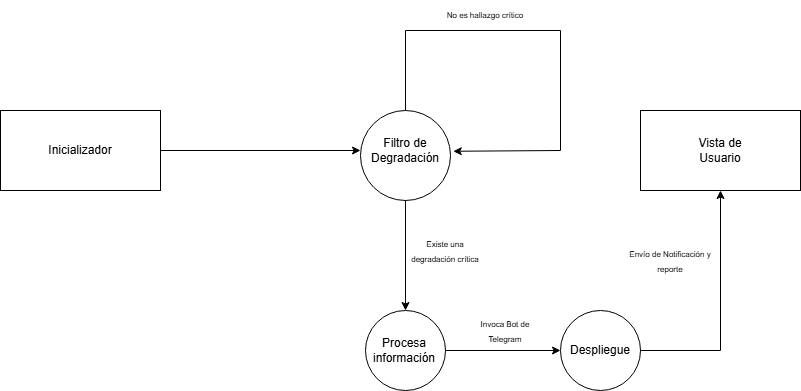
\includegraphics[width=0.8\textwidth]{Esquemas e imágenes/Modelo Navegación.png}
            \caption{Modelo de Navegación}

    \end{figure}

    \begin{itemize}
        \item \textbf{Inicializador:} El sistema comienza el proceso de evaluación de la red FTTH mediante la ejecución del modelo predictivo.
        \item \textbf{Filtro de degradación:} Es el núcleo que evalúa el modelo. Si los datos analizados determinan que "No es hallazgo crítico", el flujo se reinicia y queda a la espera de nueva información sin interrumpir al usuario.
        \item \textbf{Procesa información:} Cuando el modelo detecta que ''Existe una degradación crítica'' (como una caída anómala en la potencia óptica), los datos pasan a esta etapa para estructurar el reporte de impacto.
        \item \textbf{Despliegue: Helpdesk:} Se activa el mecanismo de comunicación, invocando la API de Zammad.
        \item \textbf{Vista de Usuario:} El flujo concluye con el ''Envío de Notificación y reporte'' donde el usuario visualiza la alerta directamente en su cliente de mensajería o correo electrónico, cerrando el ciclo de navegación de la información.  
    \end{itemize}


\subsection{Diseño de Interfaces de Usuarios}
\noindent
La interfaz de usuario final se ha diseñado pensando en la inmediatez, aprovechando la vista móvil de las aplicaciones de correo electrónico a través de la integración automatizada con Zammad. El diseño carece de elementos distractivos y prioriza una jerarquía visual orientada a la rápida asimilación de la información técnica crítica.

\begin{figure}[H]
    \centering
    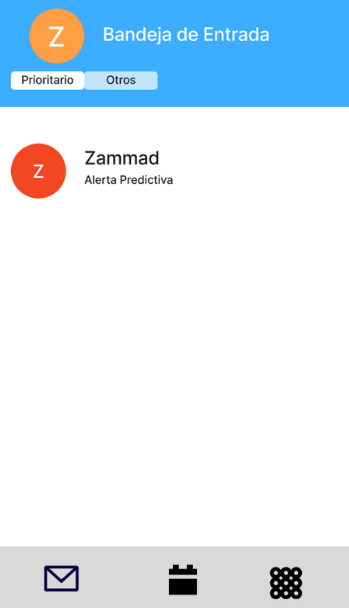
\includegraphics[width=0.4\textwidth]{Esquemas e imágenes/Interfaz 1.png}
    \caption{Vista principal de notificación preventiva de Zammad en la bandeja de entrada.}
\end{figure}

\begin{figure}[H]
    \centering
    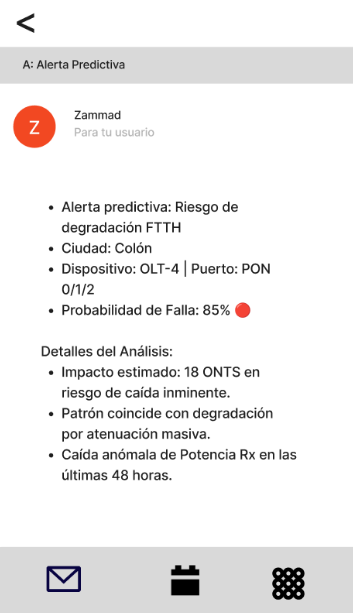
\includegraphics[width=0.4\textwidth]{Esquemas e imágenes/Interfaz 2.png}
    \caption{Reporte detallado tras la apertura de la notificación en el cliente de correo.}
\end{figure}

\begin{itemize}
    \item \textbf{Bandeja de entrada:} La alerta se identifica claramente bajo el remitente del sistema de tickets y un asunto prioritario ("Alerta predictiva"), destacándose inmediatamente frente a los correos operativos regulares.
    
    \item \textbf{Cuerpo de la Alerta:} Una vez abierto el correo, la interfaz presenta un resumen en formato de lista para agilizar la lectura técnica y la toma de decisiones:
    \begin{itemize}
        \item \textbf{Contexto de la falla:} Se especifica de inmediato el Riesgo de degradación FTTH.
        \item \textbf{Ubicación y Hardware:} Se expone la topología afectada, detallando la ciudad (Ej. Colón) y el equipo físico (Ej. Dispositivo: OLT-4; Puerto: PON 0/1/2). Esto es vital para orientar rápidamente las acciones del personal en terreno.
        \item \textbf{Métrica de riesgo:} Se destaca la probabilidad de falla mediante un porcentaje claro (Ej. 85\,\%) acompañado de un indicador visual (círculo de color) que denota la severidad de la alerta de forma intuitiva.  
    \end{itemize}

    \item \textbf{Detalles del Análisis:} Sección dedicada a la explicabilidad del modelo predictivo, fundamental para generar confianza en el usuario. Aquí se desglosa el impacto estimado (cantidad de ONTs en riesgo de caída inminente), el patrón reconocido por el modelo (ej. atenuación masiva) y la causa temporal de la anomalía detectada.
\end{itemize}



    \section{Conclusión}
\noindent
    El diseño preliminar expuesto en este documento establece una base arquitectónica robusta y viable para resolver la problemática del mantenimiento reactivo en las redes FTTH de Liberty Latinamerica.
    A través de la definición de un pipeline que abarca desde la extracción y consolidación de la telemetría proveniente de las OLT y ONT, 
    hasta la ingeniería de características y la aplicación de modelos de aprendizaje automático, se ha diseñado una solución capaz de procesar el comportamiento
    histórico de la red para la detección temprana de anomalías físicas.\\\\

    \noindent
    Uno de los mayores valores de la arquitectura propuesta radica en su enfoque operativo. La integración del modelo predictivo con los sistemas de gestión y 
    notificación (a través de la API de Zammad) asegura que la inteligencia analítica no quede aislada, sino que se traduzca de manera automática y visual en 
    alertas accionables para el despliegue de personal técnico en terreno. Esto reduce la fricción cognitiva del usuario final y agiliza los tiempos de respuesta.
    Con esta arquitectura de módulos y flujos de información ya definidos, los próximos pasos del proyecto se centrarán en la fase de prototipado y pruebas. 
    Los esfuerzos técnicos inmediatos se dirigirán en el procesamiento del volumen de datos corporativos y el tratamiento del desbalanceo de clases característico de 
    este tipo de fallas minoritarias y evaluación de algoritmos para el entrenamiento del modelo. 
    Esto garantizará que el sistema final cumpla con la precisión necesaria para reducir los costos de salidas a terreno (OpEx) y asegurar la calidad del servicio (QoS) esperada.

    %Bibliografía
\begin{thebibliography}{10}

\bibitem{slr_reliability}
H. Nurcahyanto, I. D. Irawati, G. D. Hantoro, Y. Purwanto, y M. Awaluddin, ``A Systematic Literature Review on Machine Learning for Network Reliability in Telecommunications Industry,'' \textit{IEEE Access}, vol. 13, pp. 201098-201124, Nov. 2025.

\bibitem{infinite_mixture}
A. Echraibi, J. Flocon-Cholet, S. Gosselin, y S. Vaton, ``An Infinite Multivariate Categorical Mixture Model for Self-Diagnosis of Telecommunication Networks,'' en \textit{23rd Conference on Innovations in Clouds, Internet and Networks (ICIN)}, París, Francia, 2020, pp. 258-265.

\bibitem{automated_gpon}
Z. Damoue, C. L. Adjaba, A. E. S. Biao, e I. S. Yaye, ``Automated management of optical fibers infrastructure in FTTH/GPON networks,'' en \textit{Proc. of International Conference on Electrical and Computer Engineering Researches (ICECER)}, Antananarivo, Madagascar, Dic. 2025.

\bibitem{stacking_ensemble}
Z. Sun, F. Yang, C. Zhang, D. Wang, y M. Zhang, ``A Stacking Ensemble ML-Based Failure Prediction Model for Optical Networks with Imbalanced Data,'' en \textit{2023 Asia Communications and Photonics Conference/2023 International Photonics and Optoelectronics Meetings (ACP/POEM)}, 2023.

\bibitem{shap_lime}
W. H. K. Atmaja, N. A. C. Andryani, H. Prabowo, H. Soeparno, y N. Liam, ``Predicting FTTH Take-Up Ratio in West Java Using SHAP and LIME Methods,'' en \textit{2024 3rd International Conference on Creative Communication and Innovative Technology (ICCIT)}, 2024.

\bibitem{nokia_predictive}
Nokia Corporation, ``Predictive Maintenance and Optical Analytics Framework,'' Informe Técnico. [En línea]. Disponible: \url{https://www.nokia.com/networks/services/predictive-care/}

\bibitem{vc4_predictive}
VC4 Network Lifecycle Management, ``How to Predict a Fiber Break Before It Happens: Math, Models, and Metadata,'' Artículo Técnico, Jul. 2025. [En línea]. Disponible: \url{https://www.vc4.com/blog/how-to-predict-a-fiber-break-before-it-happens/}

\bibitem{ftth_gpon_design}
Z. Abdellaoui, Y. Dieudonne, y A. Aleya, ``Design, implementation and evaluation of a Fiber To The Home (FTTH) access network based on a Giga Passive Optical Network GPON,'' \textit{Array}, vol. 10, p. 100058, 2021.

\bibitem{isp_predictive}
A. N. Philip y A. E. Aeroborman, ``Using Machine Learning for Predictive Maintenance in Fiber-based ISP Networks,'' \textit{International Journal of Modern Science and Research Technology}, vol. 3, no. 10, pp. 742-747, Oct. 2025.

\bibitem{bhais_gpon}
O. A. A. Bhais, Z. I. Mohd Yusoh, M. F. Iskandar Othman, M. Sammour, N. Bahaman, y N. Z. Syazrah Othman, ``Machine Learning-Based Proactive Fault Monitoring and Prediction in GPON Networks,'' \textit{Modern Applied Science}, vol. 19, no. 2, pp. 13-31, 2025.

\bibitem{ieee1012}
``IEEE Standard for System, Software, and Hardware Verification and Validation,'' \textit{IEEE Std 1012-2016}, IEEE, 2017.

\end{thebibliography}
\end{document}